 \documentclass[a4paper,11pt]{article}

\usepackage{amsmath}
\usepackage{amssymb}
\usepackage{amsthm}
\usepackage{graphicx}
\usepackage{caption}
\usepackage{subcaption}

\newtheorem{thm}{Theorem}
\newtheorem{lem}{Lemma}

\newcommand{\beq}{\begin{equation}}
\newcommand{\eeq}{\end{equation}}

\newcommand{\ba}{\begin{array}}
\newcommand{\ea}{\end{array}}

\newcommand{\bea}{\begin{eqnarray}}
\newcommand{\eea}{\end{eqnarray}}

\newcommand{\bc}{\begin{center}}
\newcommand{\ec}{\end{center}}

\newcommand{\ds}{\displaystyle}

\newcommand{\bt}{\begin{tabular}}
\newcommand{\et}{\end{tabular}}

\newcommand{\bi}{\begin{itemize}}
\newcommand{\ei}{\end{itemize}}

\newcommand{\bd}{\begin{description}}
\newcommand{\ed}{\end{description}}

\newcommand{\bp}{\begin{pmatrix}}
\newcommand{\ep}{\end{pmatrix}}

\newcommand{\p}{\partial}
\newcommand{\sech}{\mbox{sech}}

\newcommand{\cf}{{\it cf.}~}

\newcommand{\ltwo}{L_{2}(\mathbb{R}^{2})}
\newcommand{\smooth}{C^{\infty}_{0}(\mathbb{R}^{2})}

\newcommand{\br}{{\bf r}}
\newcommand{\bk}{{\bf k}}
\newcommand{\bv}{{\bf v}}

\newcommand{\gnorm}[1]{\left|\left| #1\right|\right|}
\newcommand{\ipro}[2]{\left<#1,#2 \right>}
\title{Nonlinear Waves over Vortices}
\author{Christopher W. Curtis\\ San Diego State University\\ Department of Mathematics and Statistics}
\date{}
\begin{document}
\maketitle
\section{Introduction}
Motivated by the need to identify moving underwater objects by their surface wave signatures, a number of authors have studied the problem of how free fluid surfaces respond to the motion of submerged vortices.  This has included detailed analytic studies of one or two vortices for short times \cite{tyvand1,tyvand2}, and numerical and experimental studies of how two counter-rotating vortices induce surface wave motion over asymptotically significant time scales \cite{marcus,telste,tryggvason}.  Collectively, this work established two regimes of vortices, the so-called `sub-critical' and `super-critical' cases characterized by the magnitude of the non-dimensional Froude number.  

In the super-critical case, the vortices move closer together while rising, inducing the formation of surface humps and `scars', or depressions.  Ultimately, in the super-critical case, these waves break.  The sub-critical case is characterized by relatively weak surface response with the vortex motion proceeding as in the case of a rigid lid.  On long enough time scales though where the vortices are able to get close enough to the surface, breaking can be seen.  However, in all of this previous work, the fluid is assumed infinitely deep and constraints are explicitly placed on the flow which keep the vortex positions symmetric.  Thus bottom boundary effects are not captured, and while there is agreement with experimental results, it is not clear on longer time scales if the symmetry restrictions used in simulation and analysis allow for the full range of relevant flows.  Complementing this work, using conformal maps and asymptotic methods, the details of how an isolated vortex over an infinitely deep fluid can induce surface wave radiation up to and past the speed of sound was studied in \cite{ruban}.       

However, motivated by the experiments in \cite{lin,liu1,liu2}, in which it is shown how surface waves induce eddy formation as they move over varying bathymetry in shallow water, we argue that there is a need to examine larger collections of vortices, and with finite depth boundaries in place.  By assuming the vortices are irrotational point vortices, and looking at larger collections of them, this provides an approximation to the behavior of larger scale eddies moving underneath surface waves.

Therefore, in a shallow-water regime, by extending the method of \cite{afm}, we derive a system of differential-integral equations which describes the surface/point vortex system for an arbitrary number of submerged vortices.  Using the Dirichlet-to-Neumann Operator (DNO) approach of \cite{craig}, we are able to develop long time numerical simulations which capture most if not all of the nonlinear interactions between the surface and the vortices, where again we can have an arbitrary number of vortices.  This is a fundamentally  different approach than has been used in previous literature.  Aside from easing the development of numerical simulations, other effects are readily included, such as stratification and constant background shear, and this is a subject of future work.  Further, the framework used in the paper allows for the ready derivation of asymptotic reductions of the full nonlinear system, and this is also a subject of future work.  

In order to connect back to previous work, we present results for a counter-rotating vortex pair in the super-critical case.  While we are able to find much of the general phenomena seen previously, we see that waves of higher amplitude form over shorter time scales due to the presence of the bottom boundary which produces an upwelling effect unseen in previous work.  This ultimately leads to the formation of large amplitude nonlinear waves with deeper scars than previously seen.  Ultimately, this appears to lead to wave breaking on much faster time scales.    

We then look at all possible cases of two pairs of counter-rotating vortices with net zero angular momentum.  While sharing some similar characteristics with the two vortex case, the added interactions slow the rise of the vortices which exhibit features of both a co-rotating and co-propagating vortex pair.  This gives rise to a wide variety of surface profiles and potential wave-breaking mechanisms that have not been studied.  While multi-vortex systems have been looked at in \cite{rouhi}, where the canonical Hamiltonian structure of collections of vortices underneath surface waves was derived,   the dynamics of multi-vortex systems were not studied in this work.  Thus our results are fundamentally new. 

%By developing greater understandings of this system, the energetics and longer time dynamics of waves moving towards beaches over eddies can be better understood.  This could have applications in wave energy extraction problems and tsunami modeling near the shore.

The outline of the paper is as follows.  The remainder of this section presents the model for the surface wave/vortex system.  Section 2 presents the extension to the method in \cite{afm} and in effect shows how the entire surface wave/vortex system can be written in terms of surface variables and vortex positions alone.  Section 3 presents the shallow water formulation of the surface wave/vortex system.  DNO expansions and the linearization of the surface wave/vortex system are derived.  Section 4 presents the results of several numerical simulations involving both two and four vortices.  Section 5 presents conclusions of this work and also further describes future directions.  
  
%%%%%%%%%%%%%%%%%%%%%%%%%%%%%%%%%%%%%%%%
\subsection{Model Formulation}
Throughout this work, we assume the fluid is inviscid and incompressible.  The only vorticity in the problem comes from a collection of irrotational point vortices submerged beneath a free fluid surface.  
\begin{figure}
\centering
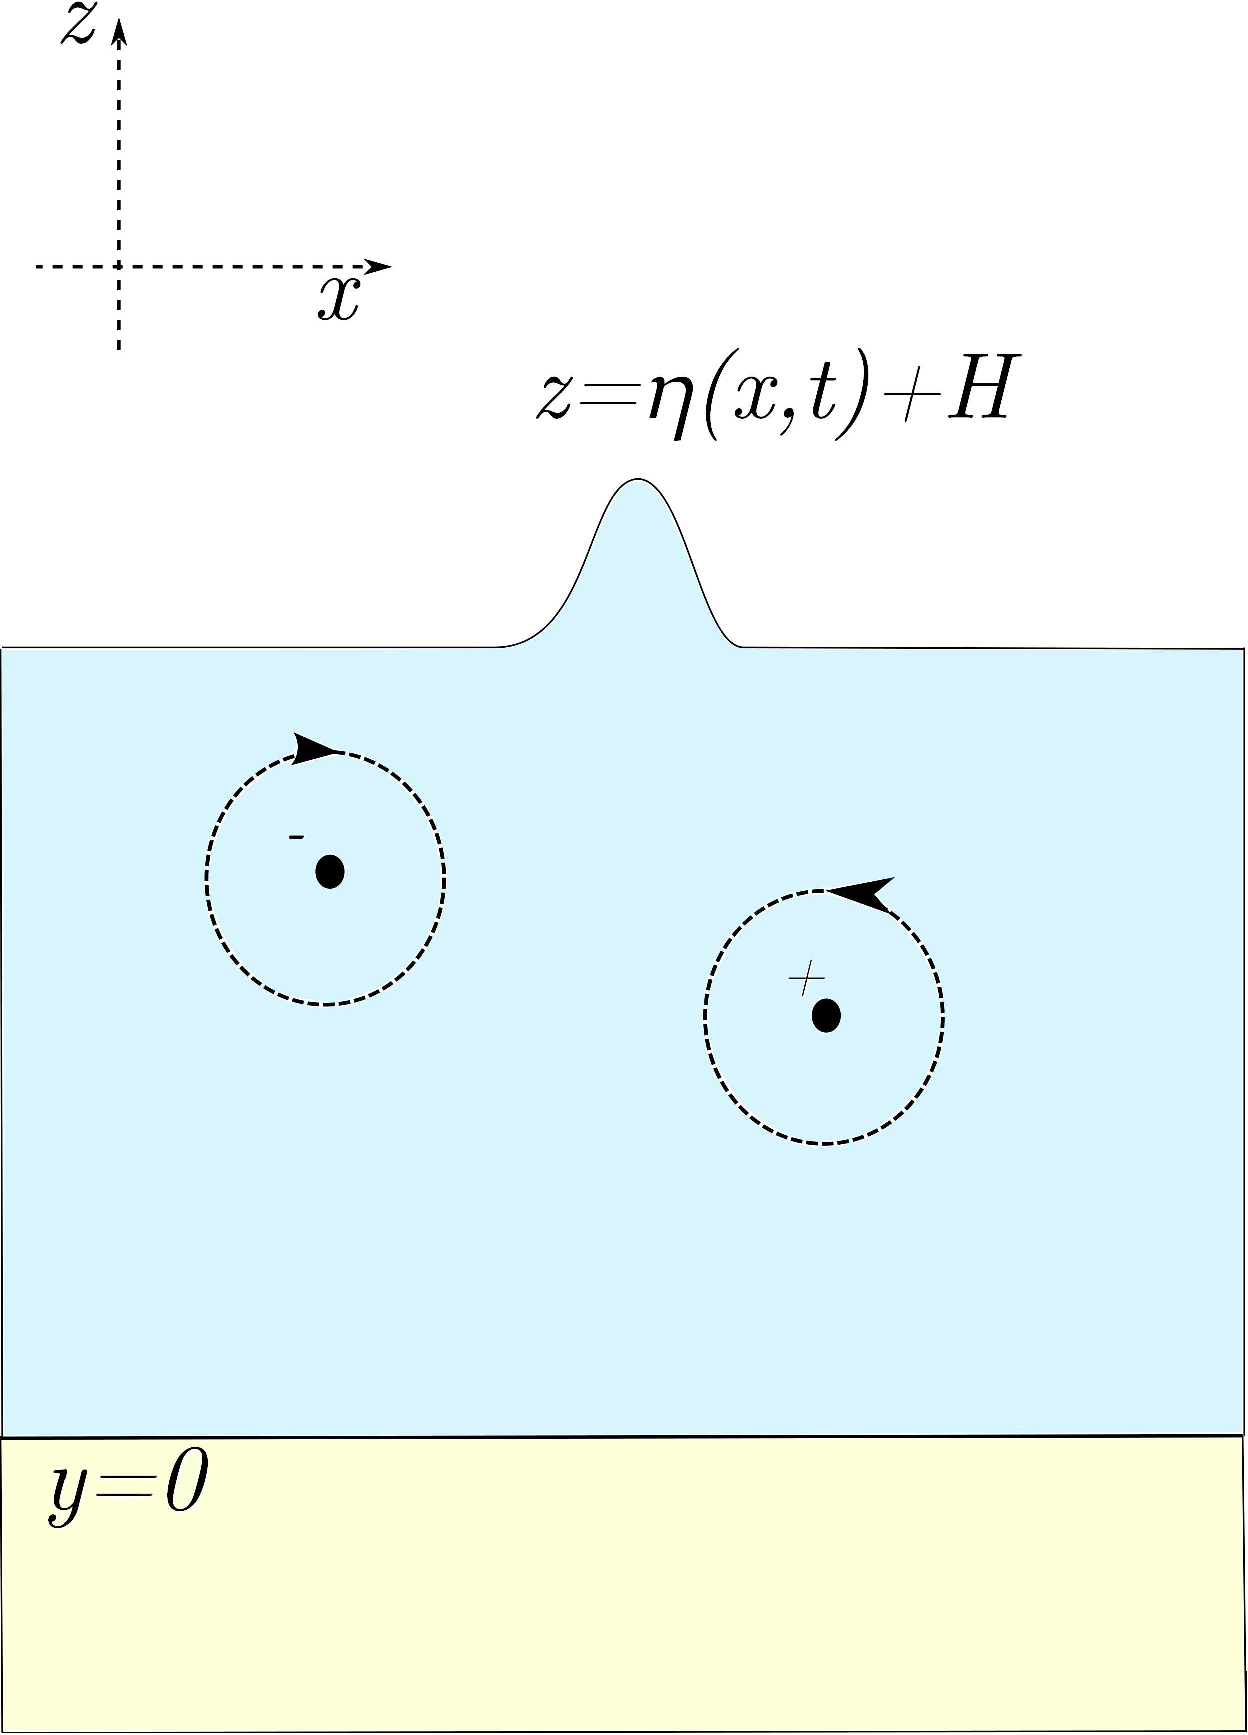
\includegraphics[width=.25\textwidth]{surface_vortex}
\caption{An irrotational point vortex submerged under a free surface gravity wave.}
\label{fig:vortex}
\end{figure}
See Figure \ref{fig:vortex} for reference.  We take the fluid domain to be periodic, with period $2L$, and $-L\leq x \leq L$.  The potential describing the flow is written as 
\[
\phi(x,z,t) = \phi_{v}(x,z,t) + \tilde{\phi}(x,z,t), 
\]
where
\[
\phi_{v}(x,z,t) = \frac{1}{2\pi}\sum_{j=1}^{N}\Gamma_{j} \phi_{v,j}(x,z,t),
\]
where $\Gamma_{j}$ denotes the circulation strength of the vortices and
\[
\phi_{v,j}(x,z,t) = \phi_{v,j}^{+}(x,z,t) - \phi_{v,j}^{-}(x,z,t), 
\]
with
\[
\phi_{v,j}^{+}(x,z,t) = \Phi_{p}(x-x_{j}(t),z-z_{j}(t)), ~ \phi_{v,j}^{-}(x,z,t) = \Phi_{p}(x-x_{j}(t),z+z_{j}(t)), 
\]
where
\[
\Phi_{p}(x,z) = \sum_{m=-\infty}^{\infty} \tan^{-1}\left(\frac{z}{x-2m L} \right).
\]
We further suppose that 
\[
\p_{z}\tilde{\phi}(x,0,t) = 0, 
\]
so that there is zero flux through the fluid bottom at $z=0$.  Thus, within the domain $0\leq z \leq \eta(x,t)+H$, we are modeling a collection of irrotational vortices underneath a moving surface. 

In order to take into account the periodically repeating images of the vortices, using Fourier transform arguments, one can show that 
\[
\sum_{m=-\infty}^{\infty}\frac{s}{(t-2m\pi)^{2}+s^{2}} = \frac{\sinh(s)}{2(\cosh(s)-\cos(t))}
\]
and
\[
\sum_{m=-\infty}^{\infty}\frac{t-2m\pi}{(t-2m\pi)^{2}+s^{2}} = \frac{\sin(t)}{2(\cosh(s)-\cos(t))}
\]
Standard arguments then give 
\begin{align*}
\dot{x}_{j} = & \frac{1}{4L}\left(  \Gamma_{j}\mbox{cotanh}\left(\frac{\pi z_{j}}{L} \right)+2\sum_{l\neq j}\Gamma_{l}v_{jl}^{(h)} \right)+ \tilde{\phi}_{x}(x_{j},z_{j},t),\\
\dot{z}_{j} = & \frac{1}{2L}\sinh\left(\frac{\pi}{L}z_{j}\right)\sum_{l\neq j} \Gamma_{l} v_{jl}^{(v)} + \tilde{\phi}_{z}(x_{j},z_{j},t),
\end{align*}
where
\begin{align*}
v_{jl}^{(h)} = & \frac{\sinh\left(\frac{\pi}{L}z_{l}\right)\left(\cosh(\frac{\pi}{L}z_{l})-\cosh(\frac{\pi}{L}z_{j})\cos\left(\frac{\pi}{L}(x_{j}-x_{l})\right)\right)}{\left(\cosh\left(\frac{\pi}{L}(z_{j}-z_{l})\right)-\cos\left(\frac{\pi}{L}(x_{j}-x_{l})\right)\right)\left(\cosh\left(\frac{\pi}{L}(z_{j}+z_{l})\right)-\cos\left(\frac{\pi }{L}(x_{j}-x_{l})\right)\right)}, \\
v_{jl}^{(v)} = & \frac{\sin\left(\frac{\pi}{L}(x_{j}-x_{l})\right)\sinh\left(\frac{\pi}{L}z_{l}\right)}{\left(\cosh\left(\frac{\pi}{L}(z_{j}-z_{l})\right)-\cos\left(\frac{\pi}{L}(x_{j}-x_{l})\right)\right)\left(\cosh\left(\frac{\pi}{L}(z_{j}+z_{l})\right)-\cos\left(\frac{\pi }{L}(x_{j}-x_{l})\right)\right)}.
\end{align*}

Likewise, we have the standard surface relations now modified by the presence of the point vortex, i.e. we have the kinematic condition 
\begin{equation}
\eta_{t} - \tilde{\phi}_{z} + \eta_{x}\tilde{\phi}_{x} =  P_{v}(x,\eta,t), ~ z =  \eta(x,t)+H,  
\label{unsckin}
\end{equation}
where
\[
P_{v}(x,\eta,t) =   \p_{z}\phi_{v} -  \eta_{x}\p_{x}\phi_{v} .
\]
and from the Bernoulli equation, we have 
\begin{equation}
\tilde{\phi}_{t} + \frac{1}{2 }\left| \nabla \tilde{\phi} \right|^{2} +  \nabla\phi_{v}\cdot \nabla\tilde{\phi} + g\eta = E_{v}(x,\eta,t),
\label{unscbern}
\end{equation}
where
\[
E_{v}(x,\eta,t) = \frac{1}{2\pi}\sum_{j=1}^{N}\Gamma_{j}\left(\dot{x}_{j}\p_{x}\phi_{v,j} + \dot{z}_{j} \p_{z}\left(\phi_{v,j}^{+} + \phi_{v,j}^{-}\right)  \right) - \frac{1}{2}\left| \nabla \phi_{v} \right|^{2}.
\]
Defining 
\[
\tilde{q}(x,t) = \tilde{\phi}(x,\eta(x,t)+H,t),
\]
we can transform the derivatives of the potential at the surface via the equations
\begin{equation}
\left.\bp\tilde{\phi}_{x}\\ \tilde{\phi}_{z}\ep\right|_{z=\eta} = \frac{1}{1+\eta_{x}^{2}}\bp 1 & \eta_{x}\\ \eta_{x} & -1\ep\bp\tilde{q}_{x} \\  -\eta_{t} + P_{v}\ep,
\label{phitrans}
\end{equation}
and
\begin{equation}
\tilde{\phi}_{t} = \tilde{q}_{t}-\tilde{\phi}_{z}\eta_{t},
\label{phittrans}
\end{equation}
%%%%%%%%%%%%%%%%%%%%%%%%%%%%%%%%%%%%%%%%%%%%%%%%%%%%%%%%%%%%%%%%%%%%%%%%%%%%%%%%%%

%%%%%%%%%%%%%%%%%%%%%%%%%%%%%%%%%%%%%%%%%%%%%%%%%%%%%%%%%%%%%%%%%%%%%%%%%%%%%%%%%%
\section{Nonlocal Formulation}
A now standard argument from \cite{afm} leads, making use of Equation \eqref{unsckin}, to the AFM equation 
\begin{equation}
\int_{-L}^{L} e^{-i\pi k x/L}\left(\cosh( k(  \eta+H))\left(\eta_{t} - P_{v} \right) + i\tilde{q}_{x}\sinh(k( \eta+H))\right) dx = 0, \label{unscafm}
\end{equation}
for $k \in \mathbb{Z}\backslash\left\{0\right\}$.  We are still left with needing to evaluate the background flow potential $\tilde{\phi}$ at the interior points $(x_{j}, z_{j})$.  To deal with this, we introduce the auxillary harmonic functions 
\[
\psi_{M,j}(x,z,t) = - \frac{1}{4\pi}\sum_{m=-M}^{M} \left( \mbox{ln}\left( \tilde{x}_{j,m}^{2} + \tilde{z}_{j,-}^{2}  \right) + \mbox{ln}\left( \tilde{x}_{j,m}^{2} + \tilde{z}_{j,+}^{2} \right)\right).
\]
where
\[
\tilde{x}_{j,m} = \frac{(x-x_{j}-2mL)}{L}, ~ \tilde{z}_{j,-} = \frac{\gamma}{H}(z-z_{j}), ~ \tilde{z}_{j,+} = \frac{\gamma}{H}(z+z_{j}),
\]
and
\[
\gamma = \frac{H}{L}.
\]

Our choice of auxillary harmonic function ensures that $\p_{z}\psi_{j}(x,0,t)=0$.  Taking $D_{\epsilon}$ to be an open bounded domain that surrounds but does not enclose the point vortices $(x_{j},z_{j})$, using Green's third identity, we have that 
\[
0 =  \int_{D_{\epsilon}}\left(\psi_{M,j}\Delta \tilde{\phi}_{x} - \tilde{\phi}_{x}\Delta\psi_{M,j} \right) dA =  \oint_{\p D_{\epsilon}} \left(\psi_{M,j}\p_{\hat{{\bf n}}}\tilde{\phi}_{x}-\tilde{\phi}_{x}\p_{\hat{{\bf n}}}\psi_{M,j} \right) ds,
\]
Note, if $\tilde{\phi}$ is harmonic, then so are all of its partial derivatives.  Defining
\[
g_{M}(x,z,t) = \psi_{M,j}\p_{\hat{{\bf n}}}\tilde{\phi}_{x}-\tilde{\phi}_{x}\p_{\hat{{\bf n}}}\psi_{M,j},
\]
We can then decompose the line integral such that 
\begin{align*}
\oint_{\p D_{\epsilon}} g_{M}(x,z,t) ds = & \int_{-L}^{L}g_{M}(x,\eta(x,t)+H,t) (1+\eta_{x}^{2})^{1/2}dx \\
& + \sum_{l=1}^{N} \oint_{C_{\epsilon}({\bf x}_{l})} g_{M} ds \\
& + \int_{0}^{\eta(x,t)+H} \left(g_{M}(L,z,t) + g_{M}(-L,z,t)\right) dz.  
\end{align*}

Taking $\epsilon \rightarrow 0^{+}$, we note that for a disc, say $C_{\epsilon}({\bf x}_{j})$  around the point vortex $(x_{j},z_{j})$ that 
\[
 \oint_{C_{\epsilon}({\bf x}_{j})} g_{M} ds =  \epsilon\int_{0}^{2\pi}\left.\left(\psi_{M,j}\p_{r}\tilde{\phi}_{x}- \tilde{\phi}_{x}\p_{r}\psi_{M,j} \right)\right|_{r=\epsilon} d\theta, 
\]
where in the disc we have 
\[
x = x_{j} + L r\cos(\theta), ~ z = z_{j} +  L r\sin(\theta).
\]
Thus, for any choice of $M>0$, we get the result 
\[
\lim_{\epsilon\rightarrow0^{+}}\oint_{C_{\epsilon}({\bf x}_{j})} \left(\psi_{M,j}\p_{\hat{{\bf n}}}\tilde{\phi}_{x}-\tilde{\phi}_{x}\p_{\hat{{\bf n}}}\psi_{M,j} \right) ds =\tilde{\phi}_{x}(x_{j},z_{j},t).
\]
Likewise, around the discs $C_{\epsilon}({\bf x}_{k})$, $k\neq j$, we have that 
\[
 \oint_{C_{\epsilon}({\bf x}_{k})} \left(\psi_{M,j}\p_{\hat{{\bf n}}}\tilde{\phi}_{x}-\tilde{\phi}_{x}\p_{\hat{{\bf n}}}\psi_{M,j} \right) ds = \epsilon\int_{0}^{2\pi}\left(\psi_{M,j}\p_{r}\tilde{\phi}_{x}- \tilde{\phi}_{x}\p_{r}\psi_{M,j} \right)d\theta, 
\]
where we now take 
\[
x = x_{k} + L r\cos(\theta), ~ z = z_{k} +  L r\sin(\theta).
\]
In this case though, each function in the integrand is continuous over the disc $C_{\epsilon}({\bf x}_{k})$, and thus as $\epsilon \rightarrow 0^{+}$, the contributions from these integrals vanish.  

After taking this $\epsilon\rightarrow 0^{+}$ limit, we now look at letting $M\rightarrow\infty$.  As defined, $\psi_{M,j}$ does not have a well defined limit, however, its derivatives are well defined in this limit, and as we show, it is well behaved along boundaries.  To see this, along $z = \eta(x,t) + H$, we have that 
\[
g_{M}(1+\eta_{x}^{2})^{1/2} = \left.\left(\psi_{M,j}\left(- \eta_{x}\tilde{\phi}_{xx}+\tilde{\phi}_{xz}\right)-\tilde{\phi}_{x}\left(-\eta_{x}\p_{x}\psi_{M,j}+\p_{z}\psi_{M,j}\right) \right)\right|_{z= \eta+H}.
\]
Using $\tilde{\phi}_{zz} = -\tilde{\phi}_{xx}$, we get the identity
\[
\p_{x}\left(\tilde{\phi}_{z}(x, \eta+H,t) \right) = -\eta_{x}\tilde{\phi}_{xx} + \tilde{\phi}_{xz}.
\]
Thus, by integration by parts and using the fact that $\tilde{\phi}(x,z,t)$ and its derivatives are assumed to be periodic in $x$, we have that 
\begin{align*}
\int_{-L}^{L}g_{M}(x,\eta(x,t)+H,t) (1+\eta_{x}^{2})^{1/2}dx = & -\int_{-L}^{L} \left.\left(\tilde{\phi}_{z}\psi^{(1)}_{M,j}+\tilde{\phi}_{x}\psi^{(2)}_{M,j}\right)\right|_{z=\eta+H}dx \\
& + \tilde{\phi}_{z}(L,\eta+H,t)\psi^{(\delta)}_{M,j}(\eta+H,t),
\end{align*}
where
\begin{align*}
\psi^{(1)}_{M,j}(x,t) = \left.\p_{x}\psi_{M,j}+ \eta_{x}\p_{z}\psi_{M,j}\right|_{z=\eta+H}, \\
\psi^{(2)}_{M,j}(x,t) = \left.-\eta_{x}\p_{x}\psi_{M,j} + \p_{z}\psi_{M,j}\right|_{z=\eta+H}, \\
\psi^{(\delta)}_{M,j}(z,t) = \psi_{M,j}(L,z,t)-\psi_{M,j}(-L,z,t).
\end{align*}
Likewise, we have that 
\begin{align*}
\int_{0}^{\eta(x,t)+H} \left(g_{M}(L,z,t) + g_{M}(-L,z,t)\right) dz = & \int_{0}^{\eta(x,t)+H} \left(\tilde{\phi}_{xx}(L,z,t)\psi^{(\delta)}_{M,j}(z,t) \right.  \\
&\left. + \tilde{\phi}_{x}(L,z,t)\psi^{(\delta,x)}_{M,j}(z,t) \right) dz, 
\end{align*}
where
\[
\psi^{(\delta,x)}_{M,j}(z,t) = \p_{x}\psi_{M,j}(L,z,t)-\p_{x}\psi_{M,j}(-L,z,t). 
\]
One can readily show that 
\[
\psi_{M,j}^{(\delta)} = \frac{1}{4\pi}\ln\left(\left(\frac{(1-\tilde{x}_{j}-2M)^{2}+\tilde{z}_{j,-}^{2}}{(1-\tilde{x}_{j}+2(M+1))^{2}+\tilde{z}_{j,-}^{2}}\right) \left(\frac{(1-\tilde{x}_{j}-2M)^{2}+\tilde{z}_{j,+}^{2}}{(1-\tilde{x}_{j}+2(M+1))^{2}+\tilde{z}_{j,+}^{2}}\right) \right),
\]
where
\[
\tilde{x}_{j} = \frac{x_{j}}{L},
\]
and thus 
\[
\lim_{M\rightarrow\infty}\psi_{M,j}^{(\delta)}(z,t) = 0.
\]
Thus, letting $M\rightarrow \infty$, we then have 
\[
\tilde{\phi}_{x}(x_{j},z_{j},t) = \int_{-L}^{L} \left.\left(\tilde{\phi}_{z}\left(\p_{x}\psi_{j}+ \eta_{x}\p_{z}\psi_{s,j}\right)+\tilde{\phi}_{x}\left(-\eta_{x}\p_{x}\psi_{j} + \p_{z}\psi_{j} \right) \right)\right|_{z=\eta+H}dx,
\]
where we define the functions $\p_{x}\psi_{j}$ and $\p_{z}\psi_{j}$ such that 
\begin{align*}
\p_{x}\psi_{j}(x,z,t) = \lim_{M\rightarrow\infty}\p_{x}\psi_{M,j}(x,z,t), \\
\p_{z}\psi_{j}(x,z,t) = \lim_{M\rightarrow\infty}\p_{z}\psi_{M,j}(x,z,t).
\end{align*}
Transforming to surface variables using Equation \eqref{phitrans} then gives
\[
\tilde{\phi}_{x}(x_{j},z_{j},t) = \int_{-L}^{L}\left.\left(\left(\eta_{t}-P_{v}\right)\p_{x}\psi_{j} + \tilde{q}_{x}\p_{z}\psi_{j} \right) \right|_{z=\eta+H} dx.
\]

Proceeding in a similar fashion for $\tilde{\phi}_{z}$, we introduce the auxillary harmonic function
\[
\tilde{\psi}_{j} = -\frac{1}{4\pi}\sum_{m=-\infty}^{\infty} \left( \mbox{ln}\left( \tilde{x}_{j,m}^{2} + \tilde{z}_{j,-}^{2}  \right) - \mbox{ln}\left( \tilde{x}_{j,m}^{2} + \tilde{z}_{j,+}^{2} \right)\right).
\]
This choice ensures that $\tilde{\psi}_{j}(x,0,t) = 0$.  Using the arguments from above, we then can find that
\[
\int_{-L}^{L}\left.\left( \tilde{\psi}_{j}\left(\eta_{x}\tilde{\phi}_{xz}+\tilde{\phi}_{xx}\right)+\tilde{\phi}_{z}\left(-\eta_{x}\p_{x}\tilde{\psi}_{j}+\p_{z}\tilde{\psi}_{j}\right) \right)\right|_{z=\eta+H} dx  = \tilde{\phi}_{z}(x_{j},z_{j},t),
\]
where we have used the fact that $\tilde{\phi}_{zz} = -\tilde{\phi}_{xx}$.  Integrating by parts then gives 
\[
\tilde{\phi}_{z}(x_{j},z_{j},t) = \int_{-L}^{L}\left.\left(-\tilde{\phi}_{x}\left(\p_{x} \tilde{\psi}_{j} + \eta_{x}\p_{z} \tilde{\psi}_{j}\right) +\tilde{\phi}_{z}\left(-\eta_{x}\p_{x} \tilde{\psi}_{j}+\p_{z}\tilde{\psi}_{j}\right)\right)\right|_{z=\eta+H}dx,
\]
which can be shown, again using Equation \eqref{phitrans}, to yield
\[
\tilde{\phi}_{z}(x_{j},z_{j},t) = \int_{-L}^{L}\left.\left( \left(\eta_{t}-P_{v}\right)\p_{z}\tilde{\psi}_{s,j} - \tilde{q}_{x}\p_{x}\tilde{\psi}_{s,j} \right)\right|_{z=\eta+H} dx.
\]
Thus, we get the following dynamical system for the motion of the vortices:
\begin{align}
\dot{x}_{j} = & \frac{1}{4L}\left(  \Gamma_{j}\mbox{cotanh}\left(\frac{\pi z_{j}}{L} \right)+2\sum_{l\neq j}\Gamma_{l}v_{jl}^{(h)} \right)\nonumber\\
&  +\int_{-L}^{L}\left.\left(\left(\eta_{t}-P_{v}\right)\p_{x}\psi_{s,j} + \tilde{q}_{x}\p_{z}\psi_{s,j} \right)\right|_{z=\eta + H} dx \label{xdotb}\\
\dot{z}_{j} = &  \frac{1}{2L}\sinh\left(\frac{\pi}{L}z_{j}\right)\sum_{l\neq j} \Gamma_{l} v_{jl}^{(v)}\nonumber\\
&  + \int_{-L}^{L}\left.\left( \left(\eta_{t}-P_{v}\right)\p_{z}\tilde{\psi}_{s,j} - \tilde{q}_{x}\p_{x}\tilde{\psi}_{s,j} \right)\right|_{z=\eta + H} dx. \label{zdotb}
\end{align}
%%%%%%%%%%%%%%%%%%%%%%%%%%%%%%%%%%%%%%%%%%%%%%%%%%%%%%%%%%%%%%%%%%%%%%%%%%%%%%%%
\section{Shallow Water Theory: Scalings and Linear Dynamics}
To build a shallow-water theory, we now choose the following non-dimesionalizations 
\[
\tilde{x} = \frac{x}{L}, ~\tilde{z} = \frac{z}{H}, ~ \tilde{t} = \frac{\sqrt{gH}}{L} t, ~ \eta = d\tilde{\eta}, ~ \tilde{\phi} = \mu L\sqrt{gH} \tilde{\tilde{\phi}},
\]
where we define the non-dimensional parameters
\[
\mu= \frac{d}{H}, ~ \gamma = \frac{H}{L},
\]
and where we define the Froude number $F$ to be 
\[
F = \frac{\Gamma}{\mu L \sqrt{gH}}.
\]
If we then define $Q = \tilde{q}_{x}$, the Bernoulli equation \eqref{unscbern} becomes, after using Equations \eqref{phitrans} and \eqref{phittrans} and then dropping tildes,  
\begin{align*}
Q_{t} + \eta_{x} + \mu\p_{x}\frac{1}{1+ \mu^{2}\gamma^{2}\eta_{x}^{2}} \left( \frac{1}{2}Q^{2} - \mu \gamma^{2}\eta_{t}\eta_{x}Q  +  \p_{x}\phi_{v} (Q + \mu\gamma\eta_{x}( P_{v}-\gamma\eta_{t}))   \right. \\
\left.\left. + \frac{1}{2}\left(P_{v}^{2}-\gamma^{2}\eta_{t}^{2} \right)+ \p_{z}\phi_{v}\left(\gamma \mu \eta_{x}Q-\left(P_{v}-\gamma \eta_{t}\right) \right) \right)\right|_{z=\mu\eta+1}= \p_{x}E_{v}(x,\mu\eta+1,t),
\end{align*}
where, in the first case,
\[
P_{v}(x,z,t) = F\sum_{j=1}^{N} \Gamma_{j} \left(\varphi_{z}(x-x_{j},z;z_{j})-\mu\gamma \eta_{x}\varphi_{x}(x-x_{j},z;z_{j}) \right),
\]
\[
\p_{z}\phi_{v}(x,z,t) =  F\sum_{j=1}^{N} \Gamma_{j}\varphi_{z}(x-x_{j},z;z_{j}),
\]
\[
\p_{x}\phi_{v}(x,z,t) = F\sum_{j=1}^{N}\Gamma_{j}\varphi_{x}(x-x_{j},z;z_{j}),
\]
\[
E_{v}(x,1+\mu\eta,t) = \left.\left(F\sum_{j=1}^{N}\Gamma_{j}\left(\dot{x}_{j}\varphi_{x}(x-x_{j},z;z_{j}) + \gamma\dot{z}_{j}\tilde{\varphi}_{z}(x-x_{j},z;z_{j}) \right) -\frac{\mu}{2}\left|\nabla\phi_{v} \right|^{2}\right)\right|_{z=1+\mu \eta}.
\]
where
\[
\varphi_{z}(x,z;z_{j}) = \frac{\sin(\pi x)\sinh(\pi \gamma z)\sinh(\pi \gamma z_{j})}{2\left(\cosh(\pi\gamma(z-z_{j}))-\cos(\pi x)\right) \left(\cosh(\pi\gamma(z+z_{j}))-\cos(\pi x)\right)},
\]
\[
\tilde{\varphi}_{z}(x,z;z_{j}) = \frac{\sin(\pi x)\left(\cosh(\pi \gamma z_{j})\cosh(\pi \gamma z)-\cos(\pi x)\right)}{2\left(\cosh(\pi\gamma(z-z_{j}))-\cos(\pi x)\right) \left(\cosh(\pi\gamma(z+z_{j}))-\cos(\pi x)\right)},
\]

\[
\varphi_{x}(x,z;z_{j}) = \frac{\sinh(\pi \gamma z_{j})\left(\cosh(\pi \gamma z_{j})-\cosh(\pi \gamma z)\cos(\pi x)\right)}{2\left(\cosh(\pi\gamma(z-z_{j}))-\cos(\pi x)\right) \left(\cosh(\pi\gamma(z+z_{j}))-\cos(\pi x)\right)}.
\]
The AFM equation \eqref{unscafm} becomes  
\begin{align}
\int_{-1}^{1} e^{-i\pi k x}\left(\cosh\left( \pi\gamma k (1 + \mu \eta)\right)\left(\eta_{t} - \frac{1}{\gamma}P_{v}(x,1+\mu\eta,t) \right) \right.\nonumber\\
\left.+i  \frac{1}{\gamma}Q\sinh\left(\pi \gamma k (1 + \mu \eta)\right)\right) dx = 0,~k\in\mathbb{Z},\label{finafm}
\end{align}
and Equations \eqref{xdotb} and \eqref{zdotb} become
\begin{align*}
\dot{x}_{j} = &\frac{F\mu}{4}\left(\Gamma_{j}\mbox{cotanh}\left(\pi \gamma z_{j} \right)+2\sum_{l\neq j}\Gamma_{l}v_{jl}^{(h)} \right)\\
&  +\mu\int_{-1}^{1}\left.\left( \left(\gamma \eta_{t}-P_{v} \right)\p_{x}\psi_{s,j} +  Q \p_{z}\psi_{s,j} \right)\right|_{z=\mu\eta + 1} dx\\
\dot{z}_{j} = & \frac{F\mu}{2\gamma}\sinh\left( \pi \gamma z_{j}\right)\sum_{l\neq j} \Gamma_{l} v_{jl}^{(v)}\\
&  +  \frac{\mu}{\gamma }\int_{-1}^{1}\left.\left( \left(\gamma \eta_{t}-P_{v}\right)\p_{z}\tilde{\psi}_{s,j} - Q \p_{x}\tilde{\psi}_{s,j} \right)\right|_{z= \mu \eta + 1} dx.
\end{align*}
%%%%%%%%%%%%%%%%%%%%%%%%%%%%%%%%%%%%%%%%
\subsection{Dirichlet-to-Neumann Expansions}
%%%%%%%%%%%%%%%%%%%%%%%%%%%%%%%%%%%%%%%%
Our choice of scaling allows us to readily generate the Dirichlet-to-Nuemann Operator (DNO) expansion.  This is done, as in \cite{craig} among many papers, by supposing that 
\[
\eta_{t} - \frac{1}{\gamma}P_{v}(x,1+\mu \eta,t) = \left(G_{0} + \mu G_{1} + \mu^{2}  G_{2} + \cdots \right)Q, 
\]
so that, using the AFM equation \eqref{finafm}, we then get 
\[
\hat{G}_{0}(k) = -\frac{i}{\gamma}\tanh(\pi \gamma k),
\]
\[
G_{1}Q = -\gamma^{2}\p_{x}G_{0}(\eta G_{0}Q) - \p_{x}(\eta Q),
\]
and, for $m\geq 1$, 
\begin{align*}
G_{m}Q = & -\sum_{j=1}^{\lfloor{m/2}\rfloor}\frac{1}{(2j)!}D^{2j}_{\gamma}\left(\eta^{2j}G_{m-2j}Q\right) \\
& - \gamma^{2}\p_{x}G_{0} \sum_{j=0}^{\lfloor{(m-1)/2}\rfloor}\frac{D_{\gamma}^{2j}}{(2j+1)!}\left(\eta^{2j+1}G_{m-2j-1}Q\right) - \frac{1}{m!}L_{m} \p_{x}D_{\gamma}^{m-1}\left(\eta^{m}Q \right),
\end{align*}
where
\[
\hat{D}_{\gamma} = \pi \gamma k,
\]
and
\[
\hat{L}_{m} = \left\{
\ba{rl}
1,  & m~\mbox{is odd}, \\
i\gamma \hat{G}_{0}(k),  & m~\mbox{is even}.
\ea
\right.
\]
%%%%%%%%%%%%%%%%%%%%%%%%%%%%%%%%%%%%%%%%
\subsection{Linear Dynamics}
%%%%%%%%%%%%%%%%%%%%%%%%%%%%%%%%%%%%%%%%
In order to get at least some short time intuition about the response of the above system, we suppose that $\mu \ll \gamma$, so that in the linear regime we have $\dot{x}_{j}\sim 0$, $\dot{z}_{j}\sim 0$, and 
\[
Q_{t} + \eta_{x} = 0,
\]
and
\[
\hat{\eta}_{t} -\hat{G}_{0}(k)\hat{Q} = F\int_{\mathbb{R}}e^{-i \pi kx} \tilde{P}_{v}dx,
\]

\[
\tilde{P}_{v} = \frac{\gamma\sqrt{2}}{\pi}\sum_{j=1}^{n}\Gamma_{j}z_{j}e^{-i\pi kx_{j}} \frac{x}{(x^{2}+\gamma^{2}(1-z_{j})^{2})(x^{2}+\gamma^{2}(1+z_{j})^{2})} .
\]
We can readily show using a contour integral argument that 
\[
\int_{\mathbb{R}}e^{-i\pi kx} \tilde{P}_{v}dx = -\frac{i}{\sqrt{2}}\sum_{j=1}^{n}\Gamma_{j} \frac{\sinh(\pi \gamma k z_{j})}{\gamma} e^{-i\pi kx_{j}-\pi \gamma |k|}. 
\]
Note, in order for this result to hold, we need to assume that $0\leq z_{j} <1$.  Thus, if we linearize around a quiescent initial condition, in frequency space, we get the leading order behavior
\begin{align*}
\bp \hat{Q}(k,t) \\ \hat{\eta}(k,t) \ep = & \hat{Q}_{0}\bp \cos(\omega(k)t)\\\frac{ \omega}{i\pi k} \sin(\omega(k)t)\ep \\
&-\frac{iF}{\sqrt{2}}\bp i\pi k(\cos(\omega(k)t)-1)/\omega(k) \\   \sin(\omega(k)t) \ep \sum_{j=1}^{n}\Gamma_{j}\frac{\sinh(\pi \gamma k z_{j})}{\gamma \omega(k)}e^{-i\pi kx_{j}-\pi \gamma |k|},
\end{align*}
where 
\[
\omega(k) = \sqrt{\frac{ \pi k \tanh(\pi \gamma k)}{ \gamma }}.  
\]
Looking at the response to forcing for the surface displacement $\eta(x,t)$, this response, say $R_{s}(x,t)$, can be found from summing across the separate responses due to each vortex.  These responses, say $R_{s,j}$ are found from the sums
\begin{align*}
R_{s,j}(x,t) = \sum_{k=1}^{\infty} \frac{\sin(\omega(k)t)}{\omega(k)}\frac{\sinh(\pi \gamma k z_{j})}{\gamma}e^{-\pi \gamma k}\sin(\pi k (x-x_{j})),
\end{align*}
so that 
\[
R_{s}(x,t) = F\sum_{j=1}^{n}\Gamma_{j}R_{s,j}(x,t).
\]
%%%%%%%%%%%%%%%%%%%%%%%%%%%%%%%%%%%%%%%%%%%%%%%%%%%%%%%%%%%%%%%%%%%%%%%%%%%%%%%%
\section{Numerical Results}
%%%%%%%%%%%%%%%%%%%%%%%%%%%%%%%%%%%%%%%%%%%%%%%%%%%%%%%%%%%%%%%%%%%%%%%%%%%%%%%%
For all of the following simulations, we use a pseudo-spectral in space and fourth order Runge-Kutta in time method of lines, and choose $\mu=.2$, $\gamma = \sqrt{\mu}$. 
The domain is sampled with $K_{M} = 256$ modes giving a grid spacing of $\delta x = 1/128$, while the time step used is $\delta t = 5\times 10^{-3}$, which introduces error on the order of $10^{-11}$.  The Orszag ``2/3-rule'' is used to control aliasing error throughout the simulation.      

For those problems involving only two vortices, we use the initial positions
\[
x_{1}(0)=-\mu\gamma, ~x_{2}(0)=\mu\gamma, ~z_{1}(0)=z_{2}(0)=.25.
\]
This is done since $d/L=\mu\gamma$, and thus these initial positions are consistent with our scaling assumptions.  For those problems involving four vortices, we set 
\begin{align*}
x_{1}(0)=-2\mu\gamma-\mu\gamma/2, ~ x_{2}(0)=-2\mu\gamma+\mu\gamma/2,\\ x_{3}(0)=2\mu\gamma-\mu\gamma/2, ~ x_{4}(0)=2\mu\gamma+\mu\gamma/2,
\end{align*}
and $z_{j}(0)=.25$.  Throughout, we keep $|\Gamma_{j}|=1$ and use the Froude number $F$ to set the effective strength of the vortices.  

It is nontrivial at this point to describe what choices of $F$ correspond to subcritical or supercritical vortices as described in the previous literature.  We note that our choice of $F$ is not the same as in for example \cite{tyvand1} or \cite{telste}, where they define the Froude number $\tilde{F}$ to be  
\[
\tilde{F} = \frac{\Gamma}{d^{3/2}g^{1/2}}.
\] 
Comparing these two choices of Froude number shows our choice for $F$ satisfies the equation 
\[
F = \gamma\sqrt{\mu}\tilde{F}.
\]  
The supercritical or strong case is usually taken to be when $\tilde{F}\geq 1$, which corresponds to $F\geq .2$ using the values for $\mu$ and $\gamma$ from above.  However, the distinction between sub and supercritical is better defined by phenomena, whereby in the subcritical case, the motion of surface waves has a strong influence on vortex motion, and in the supercritical case, the vortex motion drives surface wave dynamics.  Thus, throughout most of the simulations, we choose $F=.2$, but we take care to try to describe the relative strength of the vortex system based on the observed dynamics.  

For each simulation, there is of course the question of where to truncate the DNO expansions.  We use the convention of taking enough terms, say $\tilde{N}$, such that, using the numerically computed solution for $Q(x,t_{f})$, where $t_{f}$ is the final time a given simulation is run to, we satisfy the criteria  
\[
\frac{\gnorm{G_{\tilde{N}} Q}_{2}}{\gnorm{Q}_{2}} \leq \mbox{eps},
\]
where $\mbox{eps}$ denotes machine precision, which on 64-bit machines is on the order of $10^{-16}$.  We argue that satisfying this inequality should in most cases imply subsequent terms should have little to no effect on the dynamics.  However, throughout each simulation, multiple truncation points were chosen to see what impact they had on dynamics, and in all cases, no effect was seen by including terms beyond what would be selected via our truncation convention.

This argument though of course relies on the choice of $t_{f}$.  Throughout each simulation, $t_{f}$ is chosen such that running the simulation to any later time results in the numerical method becoming invalid.  This is in all cases due to the presence high frequencies with relatively large amounts of energy in these modes.  Traditionally, such phenomena is associated with a breakdown in the regularity of the solution, and for this reason, we can think of $t_{f}$ as the time at which surface waves break.  

We note that this is a heuristic measurement, and more sophisticated simulations would need to be done to establish at what times vertical gradients in the wave profile formed.  That breaking could occur is not surprising, especially as the vortices get closer to the surface.  Further, breaking has been observed in the deep water simulations reported on previously.  However, a key characteristic of shallow water flow appears to be that the onset of breaking happens far more rapidly and when the vortices are not necessarily close to the surface in distinction to the deep water case.     
%%%%%%%%%%%%%%%%%%%%%%%%%%%%%%%%%%%%%%%%%%%%%%%%%%%%%%%%%%%%%%%%%%%%%%%%%%%%%%%%
\subsection*{Two Counter Propagating Vortices under a Traveling Wave}
By setting the vortex strengths, or taking the Froude number $F$ to zero, we would expect to limit onto the classical case of shallow water flow in which the KdV equation becomes a valid asymptotic approximation.  Expanding up to $\mathcal{O}(\mu,\gamma^{2})$ we get the system of equations 
\[
\tilde{Q}_{t} + \eta_{x} + \frac{\mu}{2}\p_{x}Q^{2} \sim 0, 
\]
and
\[
\left(1 - \frac{\gamma^{2}}{2}\p_{x}^{2}\right)\eta_{t} + \p_{x}\left(1-\frac{\gamma^{2}}{6}\p_{x}^{2} \right)Q + \mu \p_{x}(\eta Q) \sim 0.
\]
By introducing the coordinates
\[
\xi = x - \tilde{t}, ~ \tau = \mu \tilde{t}, 
\]
and taking the balance 
\[
\mu = \gamma^{2}, 
\]
allows us to derive the Korteweg-de Vries (KdV) equation
\[
2Q_{\tau} + 3QQ_{\xi} + \frac{1}{3} Q_{\xi\xi\xi} = 0.
\]
Note, we see by deriving this equation that we are in fact, in the abscence of vortices, in a classicaly defined shallow water regime, thus justifying our choice of scalings {\it a posteori}.  

As is known, the KdV equation has an infinite number of periodic traveling wave solutions of the form 
\[
Q(x,t) \sim \frac{4}{3} \tilde{m}^{2}\mathcal{K}^2(\tilde{m})\mbox{cn}^{2}\left(\mathcal{K}(\tilde{m}) \left( x- t - \frac{2}{3}\mu\mathcal{K}^{2}(\tilde{m}) (2\tilde{m}^{2}-1)t\right);\tilde{m}\right),
\]
where $0\leq \tilde{m}<1$ is the elliptic modulus of the cnoidal function $\mbox{cn}(\cdot;\tilde{m})$ and where $\mathcal{K}(\tilde{m})$ represents the complete elliptic integral of the first kind.  This then implies that the surface profile is to leading order given by 
\[
\eta(x,t) \sim \left(1+\frac{2}{3}\mu \mathcal{K}^{2}(\tilde{m})(2\tilde{m}^{2}-1)\right)Q(x,t).
\]
Taking then the elliptic modulus $\tilde{m}=.2$, we look at the case of two counter-propagating vortices under the traveling wave where we set $F=.02$.  We truncate the DNO expansion at the 32nd term, i.e. $G_{31}$.    

As can be seen from the motion of the vortices in Figures \ref{fig:cnxtrackpt1} and \ref{fig:cnztrackpt1}, for short times, the relatively weak circulations cause the vortices to oscillate.  However, on a longer time scale, the vortices begin to rise, though the oscillatory motion induced in the fluid column by the passing wave causes the vortices to continue to have an oscillatory component to their motion.  We likewise see that the rightward propagation of the wave pushes the vortices along with the wave crest.  %This type of behavior is characteristic of weak vortices, and is similar to the sub-critical phenomena seen in \cite{tyvand2}.
\begin{figure}[!h]
\centering
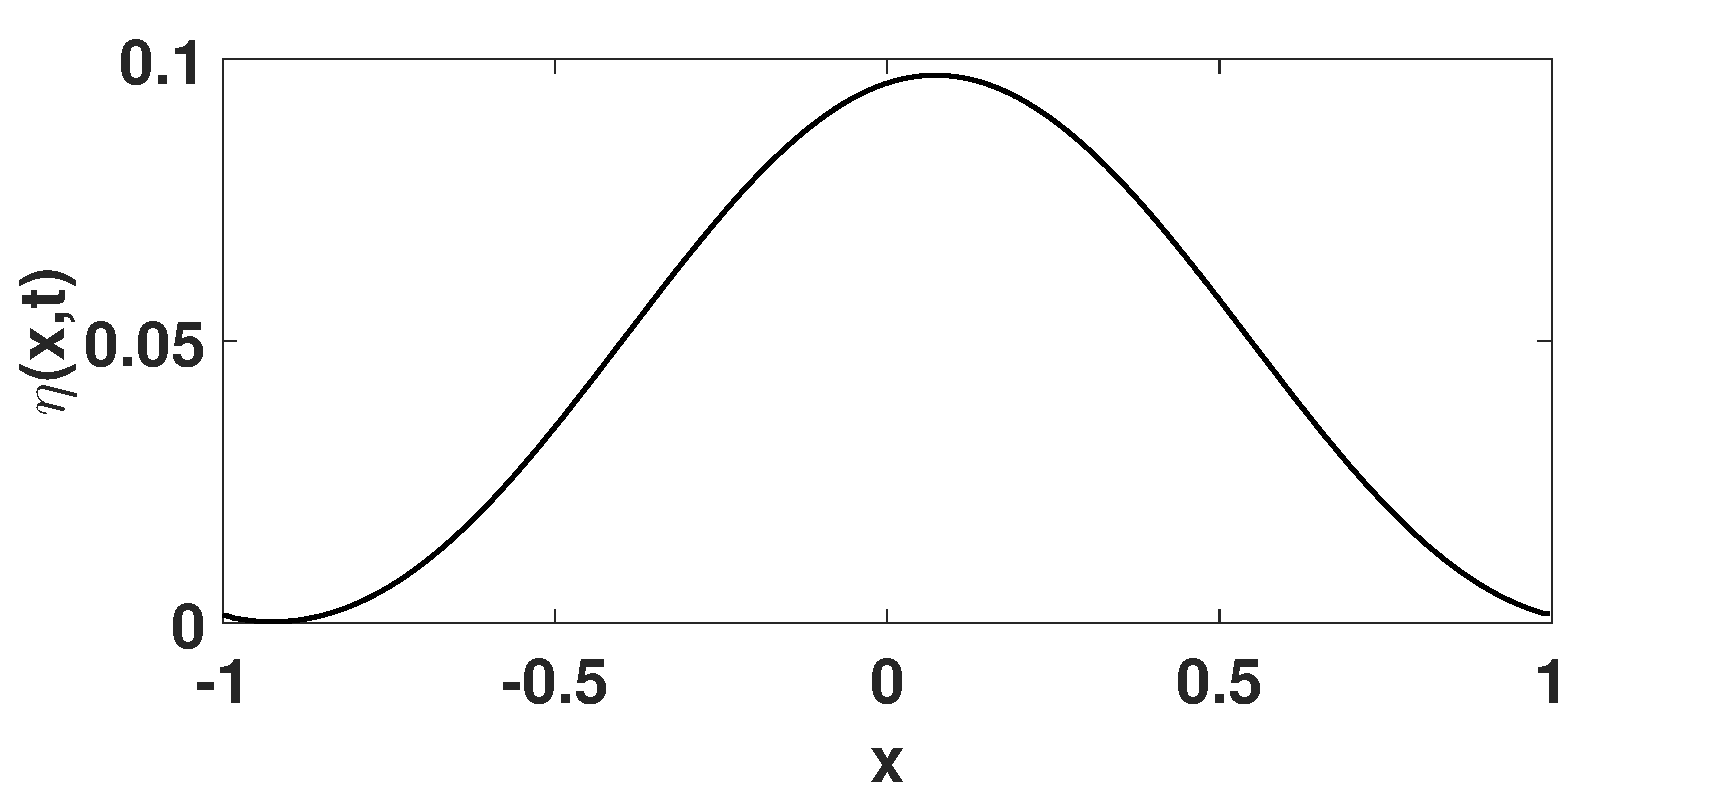
\includegraphics[width=.75\textwidth]{surf_resp_cnoid_mu_pt2_F_pt02_tf_5}
\caption{Surface response $\eta(x,5)$ for a traveling cnoidal solution of the KdV equation with elliptic modulus $\tilde{m}=.2$.}
\label{fig:surfrepcn}
\end{figure}
\begin{figure}[!h]
\centering
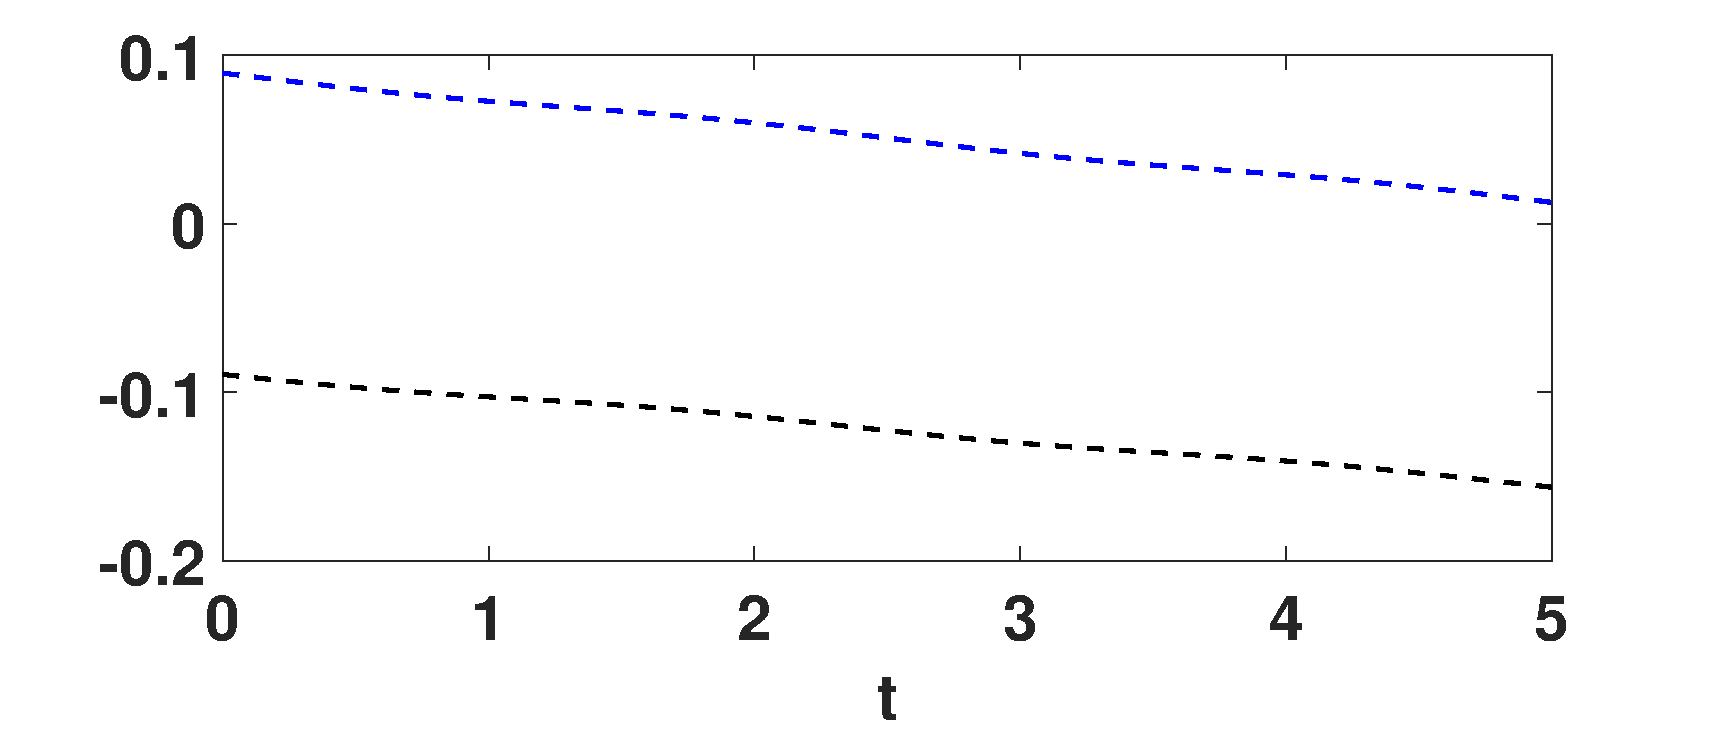
\includegraphics[width=.75\textwidth]{xtrack_cnoid_mu_pt2_F_pt02_tf_5}
\caption{Horizontal positions of vortices underneath a traveling cnoidal solution of the KdV equation for $0\leq t \leq 5$.}
\label{fig:cnxtrackpt1}
\end{figure}
\begin{figure}[!h]
\centering
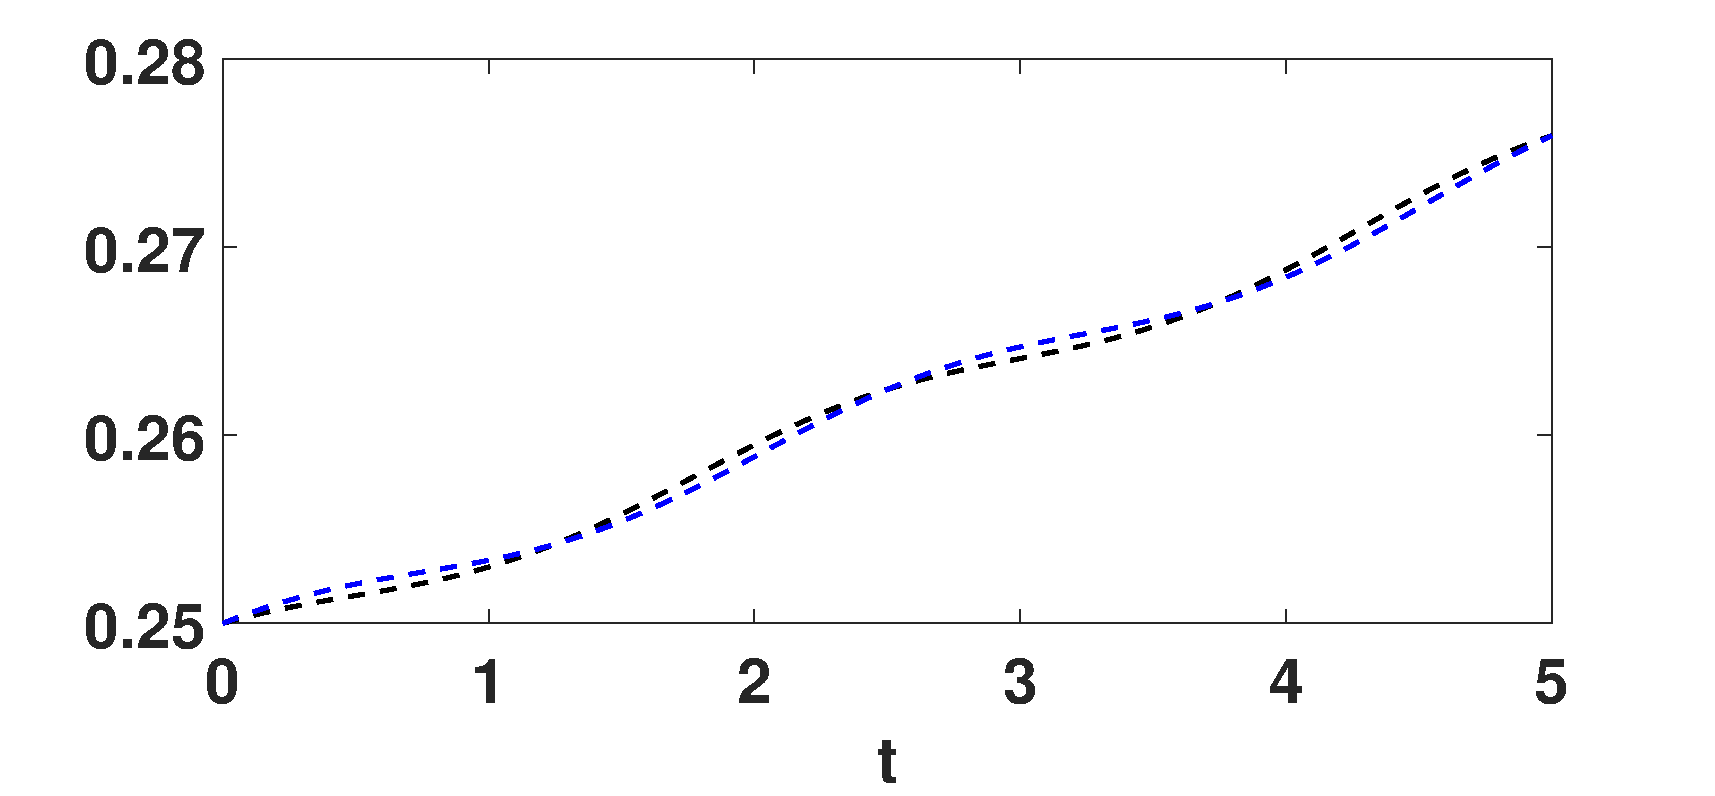
\includegraphics[width=.75\textwidth]{ztrack_cnoid_mu_pt2_F_pt02_tf_5}
\caption{Vertical position of vortices underneath a traveling cnoidal solution of the KdV equation for $0\leq t \leq 5$.}
\label{fig:cnztrackpt1}
\end{figure}

%%%%%%%%%%%%%%%%%%%%%%%%%%%%%%%%%%%%%%%%%%%%%%%%%%%%%%%%%%%%%%%%%%%%%%%%%%%%%%%%%%
\subsection*{Two Counter Propagating Vortices}
Throughout the remainder of the paper, use the initial conditions
\[
\eta(x,0) = 0, ~ 	Q(x,0) = -\p_{x}\phi_{v}(x,1),
\]
so that the initial surface profile is flat and still.  We then set $F=.2$.  

We first look at the surface response up to $t=.5$.  Given the relatively short time scale, we compare our numerics to the linear theory derived in the previous section.  For a pair of counter-rotating vortices, we have that the forcing response for the free surface is given by the function
\[
R_{s}(x,t) = 2\sum_{k=1}^{\infty} \frac{\sin(\omega(k)t)}{\omega(k)}\frac{\sinh(\pi \gamma k z_{1})}{\gamma}e^{-\pi \gamma k}\sin(\pi k x_{1})\cos(\pi k x).
\]

We compare this response function to the numerical results in Figure \ref{fig:linrep}.  As can be seen, even up to $t=.5$, the linear response is quite accurate.  Further, the falling troughs, or scars, seen in much of the existing literature \cite{marcus,tryggvason} are present.  However, we note that in previous work, the formation of mounds in the surface profile corresponded to the vortices being near the wave crest.  This is not the case in this figure as will be explained in the following paragraphs.  Thus, the presence of the bottom boundary and the concominant upwelling it induces causes wave profiles to form at far shorter time scales and for different reasons than reported in previous literature.  
\begin{figure}[!h]
\centering
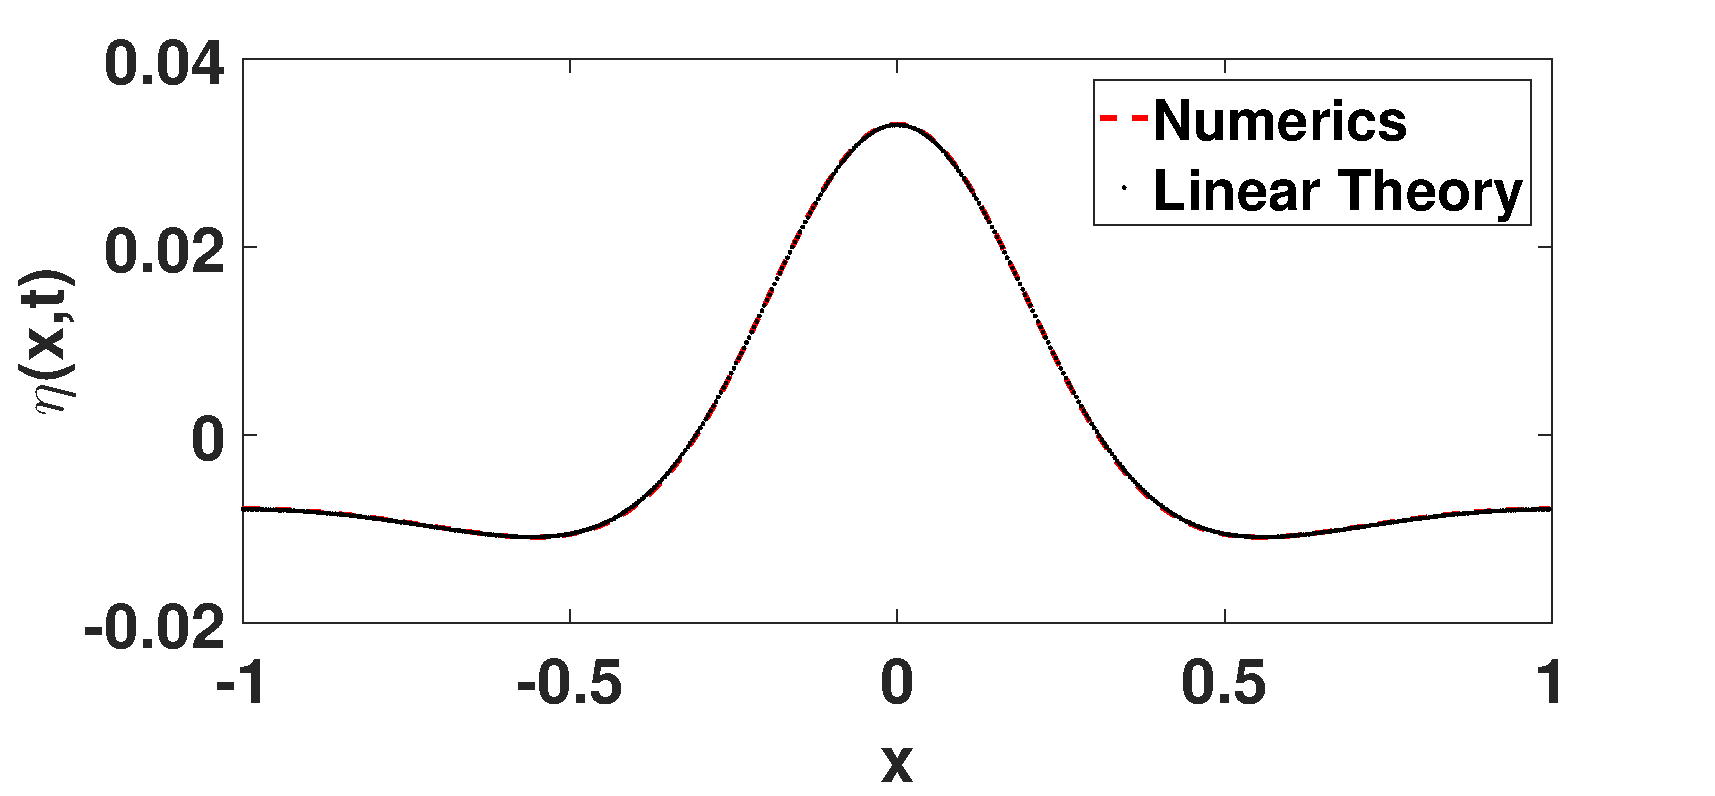
\includegraphics[width=.75\textwidth]{lin_response_tf_pt5}
\caption{Comparison between linear theory and numerics at $t=.5$ for Froude number $F=.2$.}
\label{fig:linrep}
\end{figure}

To further explore the role of nonlinearity, we now look at longer timescales where we let time $t = 6.4 \sim 32 F$.  We truncate the DNO expansions at the 19th term, i.e. $G_{18}$.  Looking at the power spectra at $t=6.4$, see Figure \ref{fig:pspecFpt2}, we see that a significant amount of energy has been transported into higher wave numbers as the vortices rise.  This explains the formation of the `jagged' scars seen in Figure \ref{fig:surfrepFpt2}, which represents the onset of wave-breaking.  Longer time simulations show that after $t=6.4$, the numerical method breaks down with the appearance of ever higher frequency oscillations, which confirms that the wave would break in physical settings.  
\begin{figure}[!h]
\centering
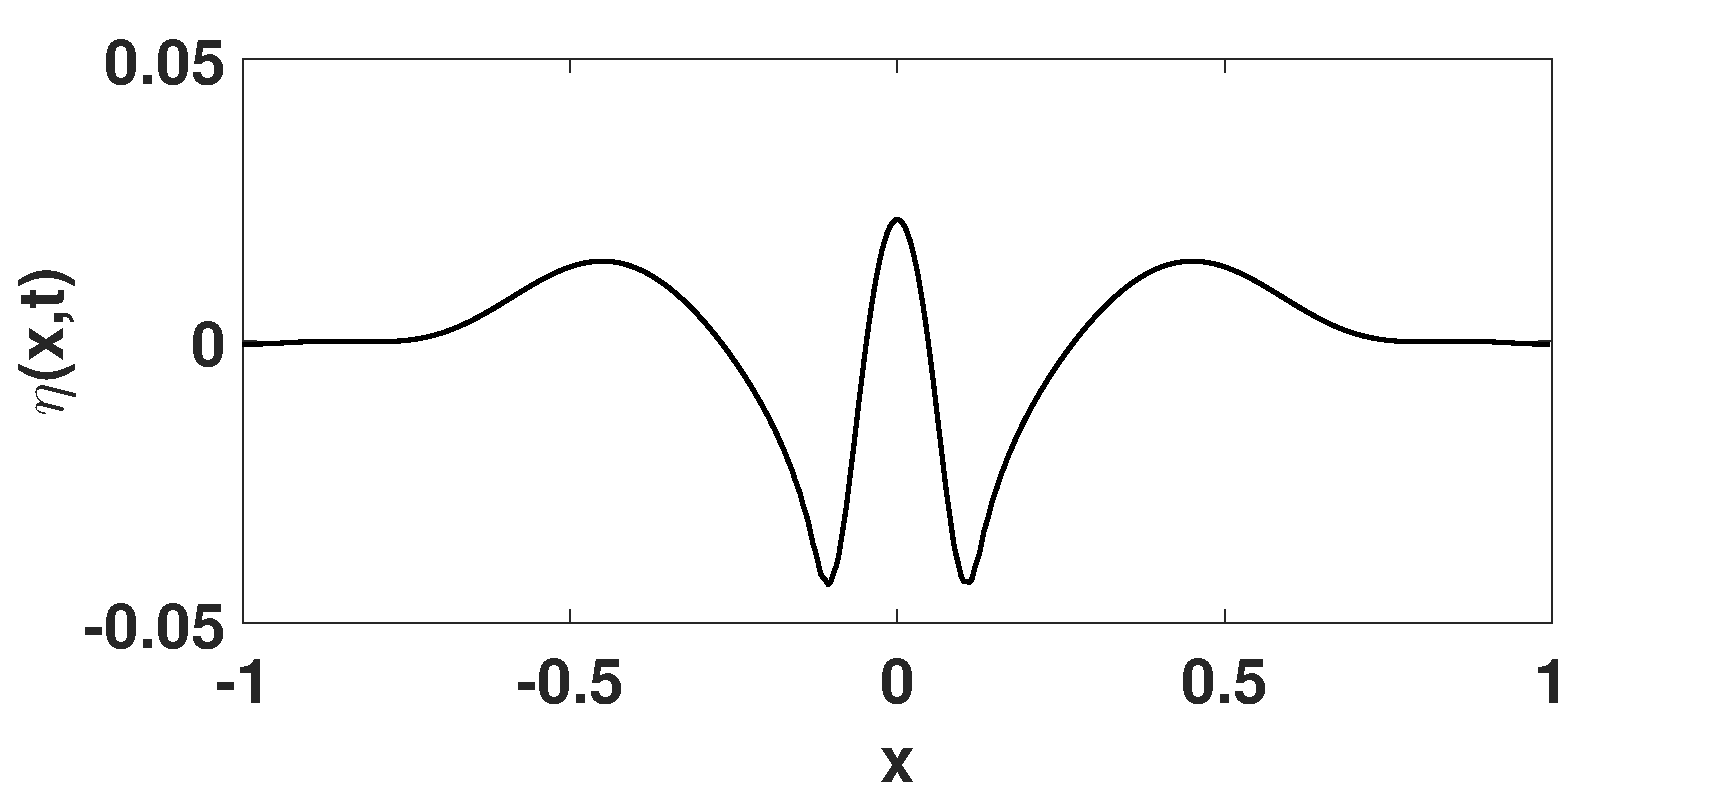
\includegraphics[width=.75\textwidth]{surf_resp_mu_pt2_F_pt2_tf_6pt4}
\caption{Surface response $\eta(x,6.4)$ over two counter-propagating vortices for small Froude number $F=.2$.}
\label{fig:surfrepFpt2}
\end{figure}
\begin{figure}[!h]
\centering
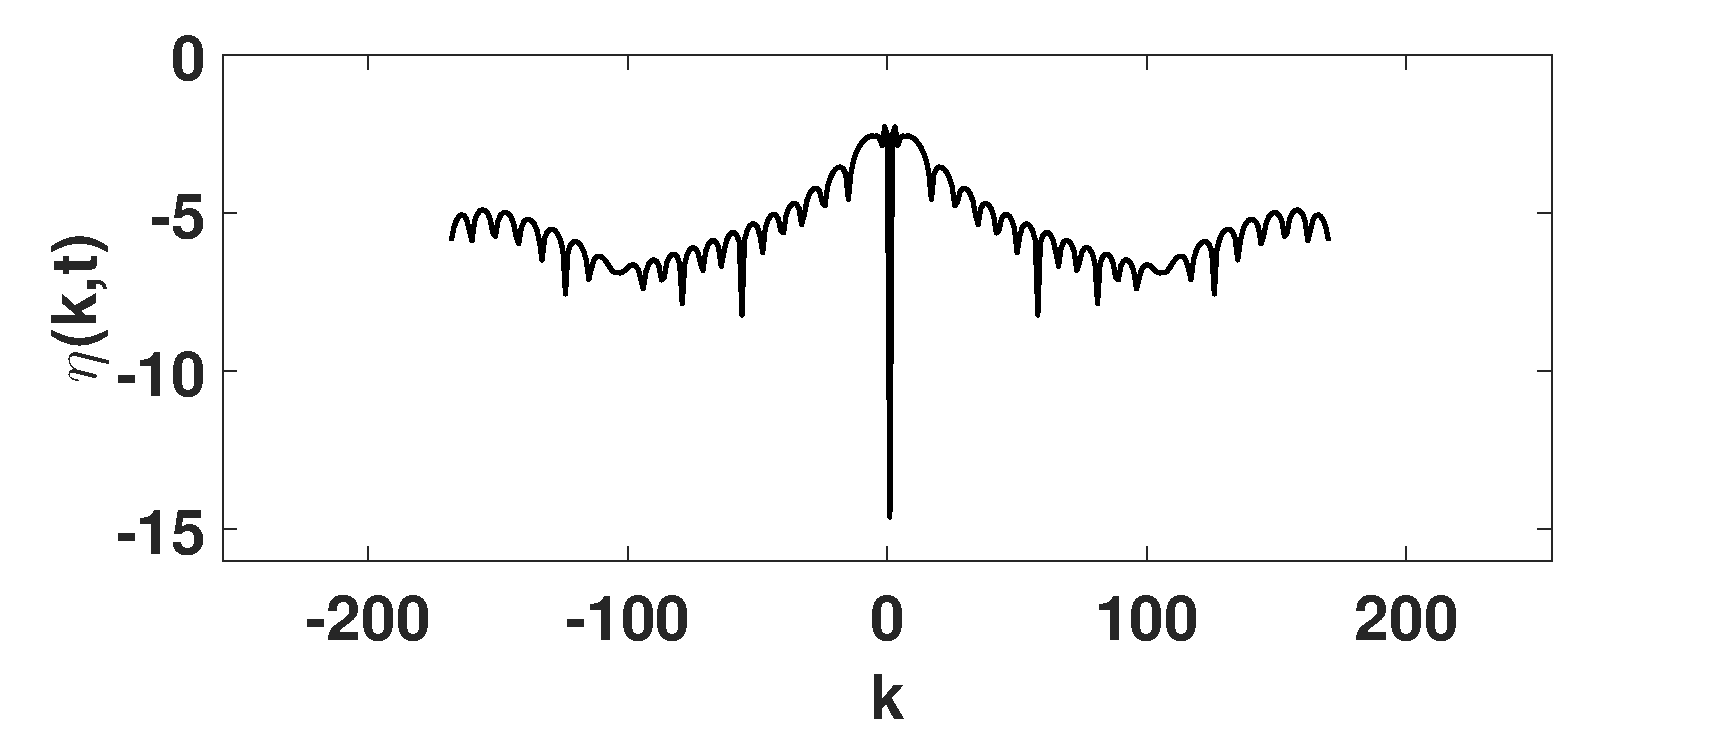
\includegraphics[width=.75\textwidth]{pspec_mu_pt2_F_pt2_tf_6pt4}
\caption{Log plot of the power spectrum at $t = 6.4$ over wave numbers $-256\leq k \leq 256$ with small Froude number $F=.2$.  As can be seen, the rising vortices pump more energy into higher wavenumbers in the surface profile.}
\label{fig:pspecFpt2}
\end{figure}
\begin{figure}[!h]
\centering
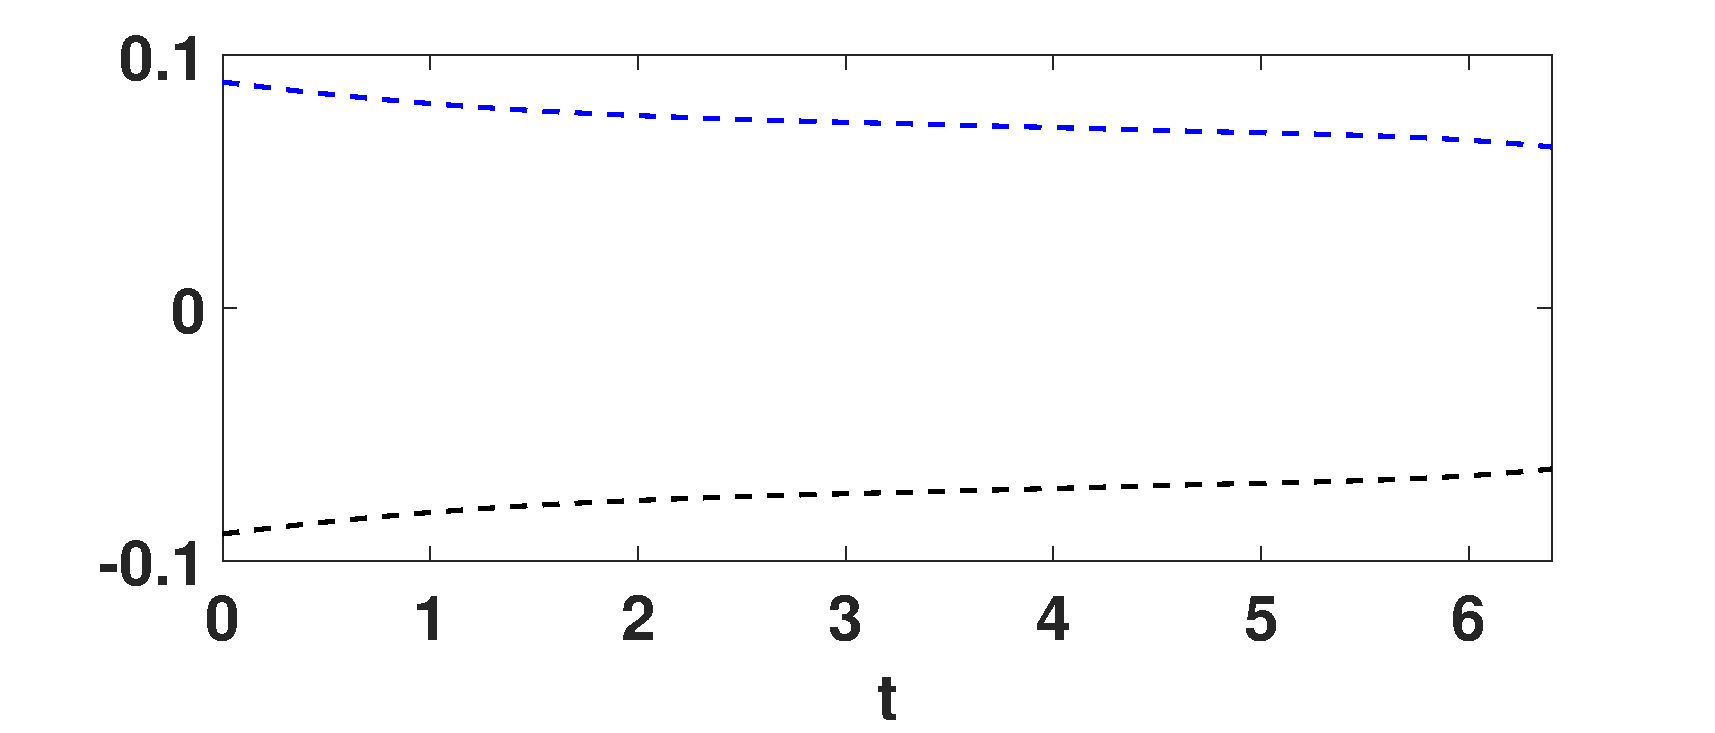
\includegraphics[width=.75\textwidth]{xtrack_mu_pt2_F_pt2_tf_6pt4}
\caption{Horizontal positions of the two vortices for $0\leq t \leq 6.4$ for small Froude number $F=.2$.}
\end{figure}
\begin{figure}[!h]
\centering
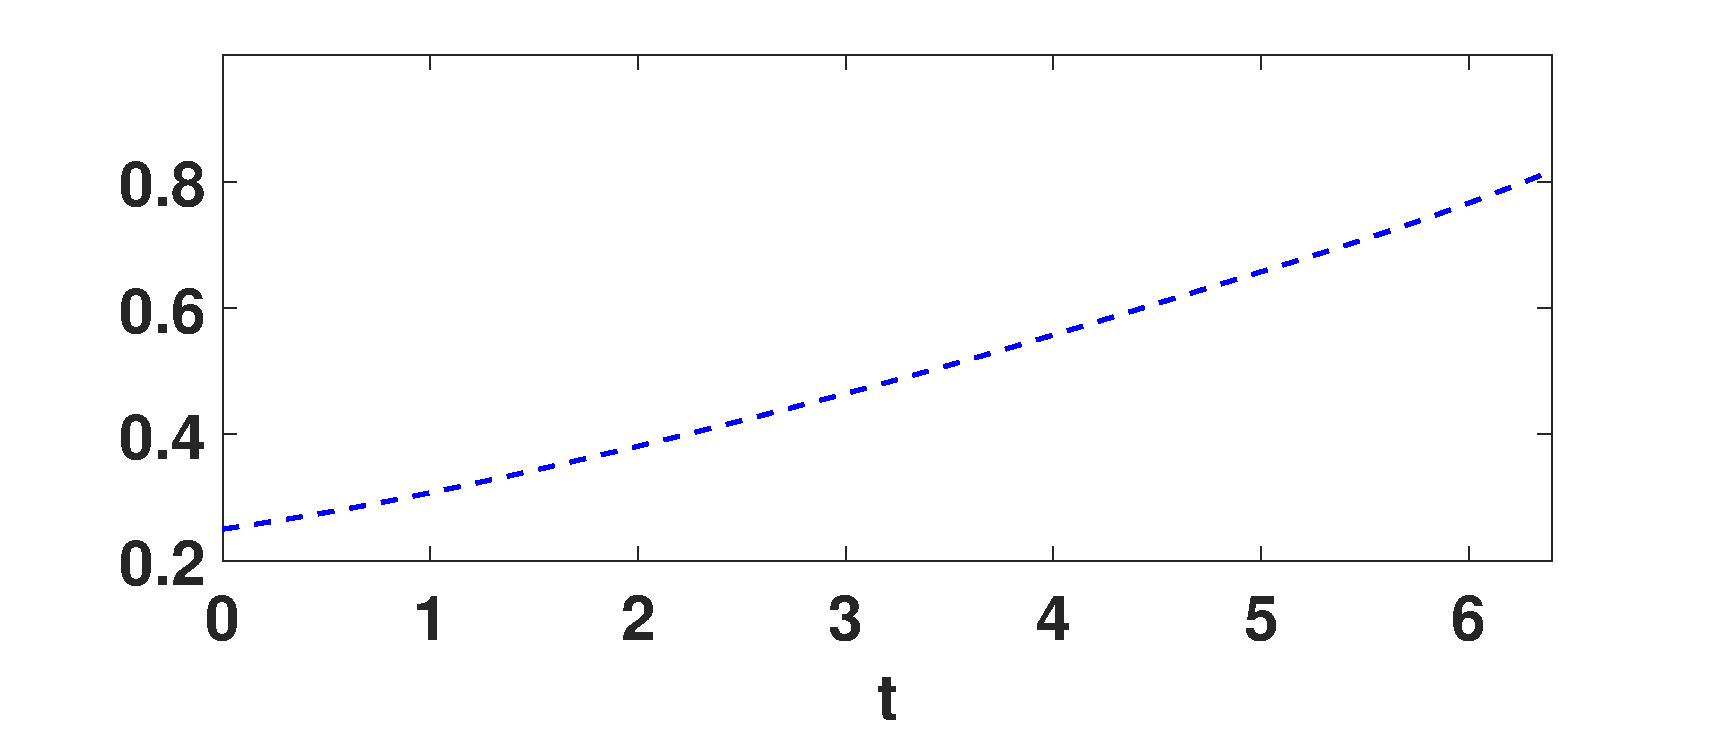
\includegraphics[width=.75\textwidth]{ztrack_mu_pt2_F_pt2_tf_6pt4}
\caption{Vertical position of the two vortices for $0\leq t \leq 6.4$ for small Froude number $F=.2$.}
\end{figure}

Given how long simulations were able to run in comparison to the Froude number, we might characterize the choice $F=.2$ as subcritical.  It is interesting then to look at the case of stronger vortices whereby we set $F=1$.  In this case the longest time we can run the simulation to before high frequencies cause the method to fail is $t_{f} = .5 \sim F/2$.  We truncate the DNO expansion at the 62nd term.  By looking at the power spectra at $t_{f}=.5$, see Figure \ref{fig:pspecF1}, we see that a significant amount of energy has been transported into higher wave numbers as the vortices rise, and while a similar phenomena is present in the $F=.2$ case, the timescales for $F=1$ are radically shorter.  
\begin{figure}[!h]
\centering
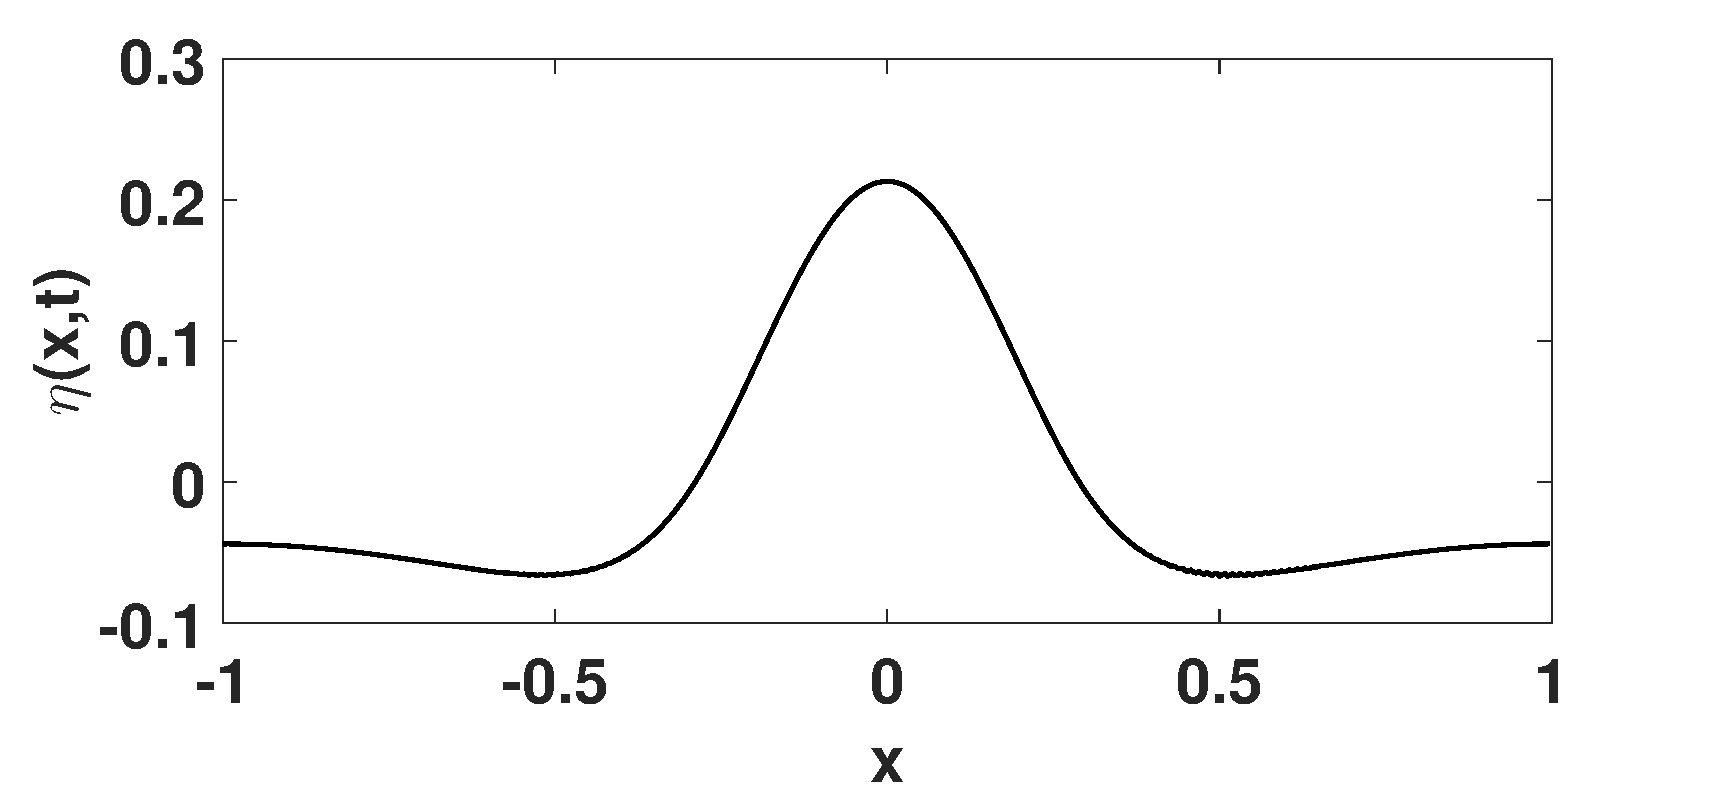
\includegraphics[width=.75\textwidth]{surf_resp_mu_pt2_F_1_tf_pt5}
\caption{Surface response $\eta(x,.5)$ over two counter-propagating vortices for large Froude number $F=1$.}
\label{fig:surfrepF1}
\end{figure}
\begin{figure}[!h]
\centering
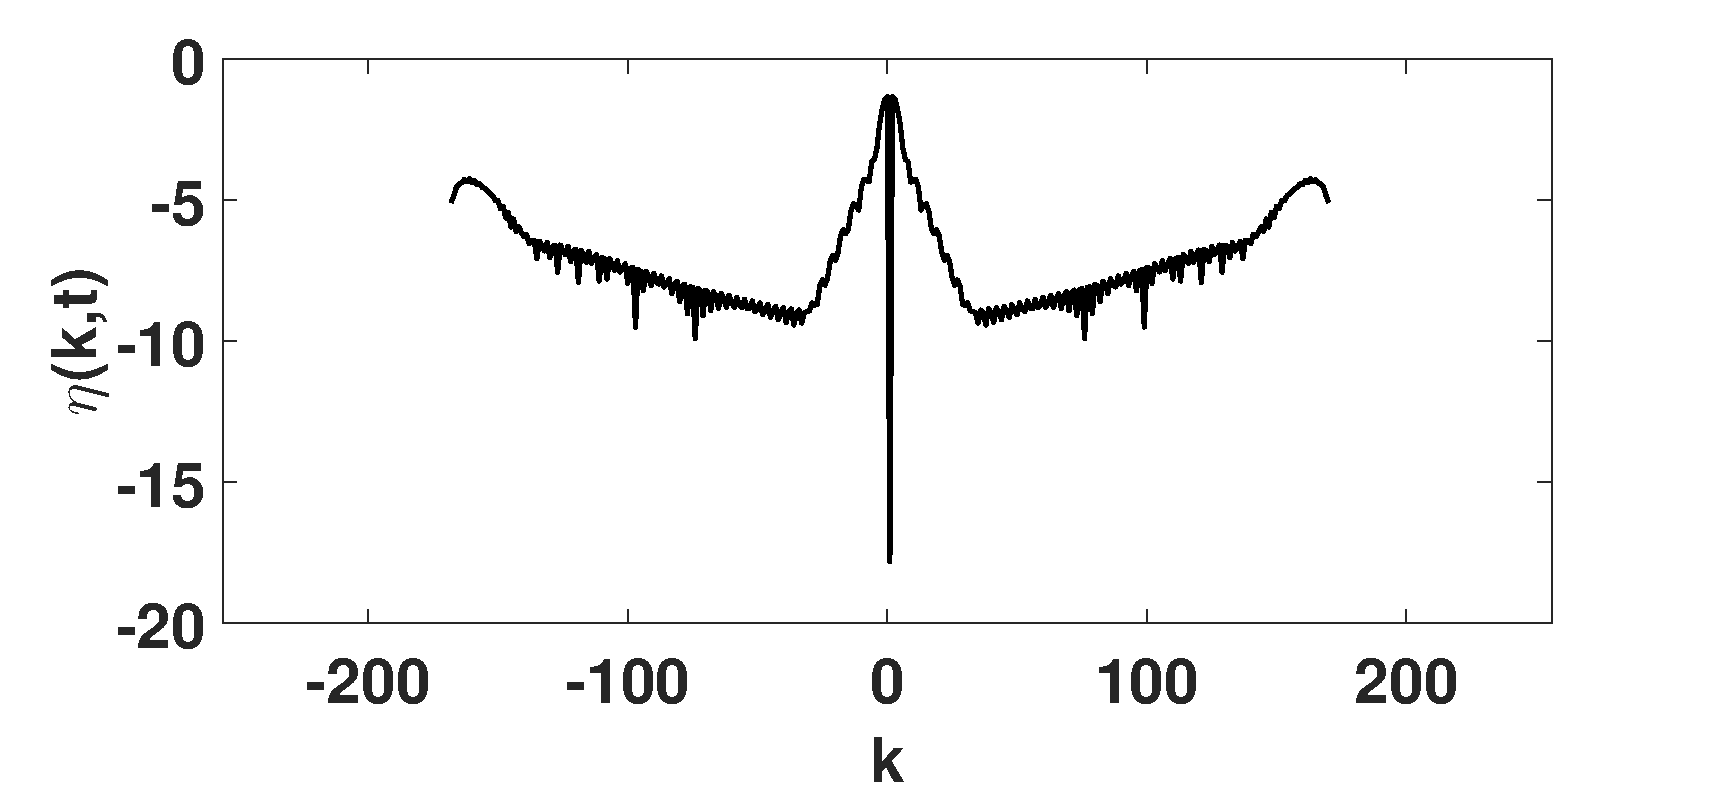
\includegraphics[width=.75\textwidth]{pspec_mu_pt2_F_1_tf_pt5}
\caption{Log plot of the Fourier transform of $\eta(x,.5)$ over wave numbers $-256\leq k \leq 256$ for large Froude number $F=1$.}
\label{fig:pspecF1}
\end{figure}
\begin{figure}[!h]
\centering
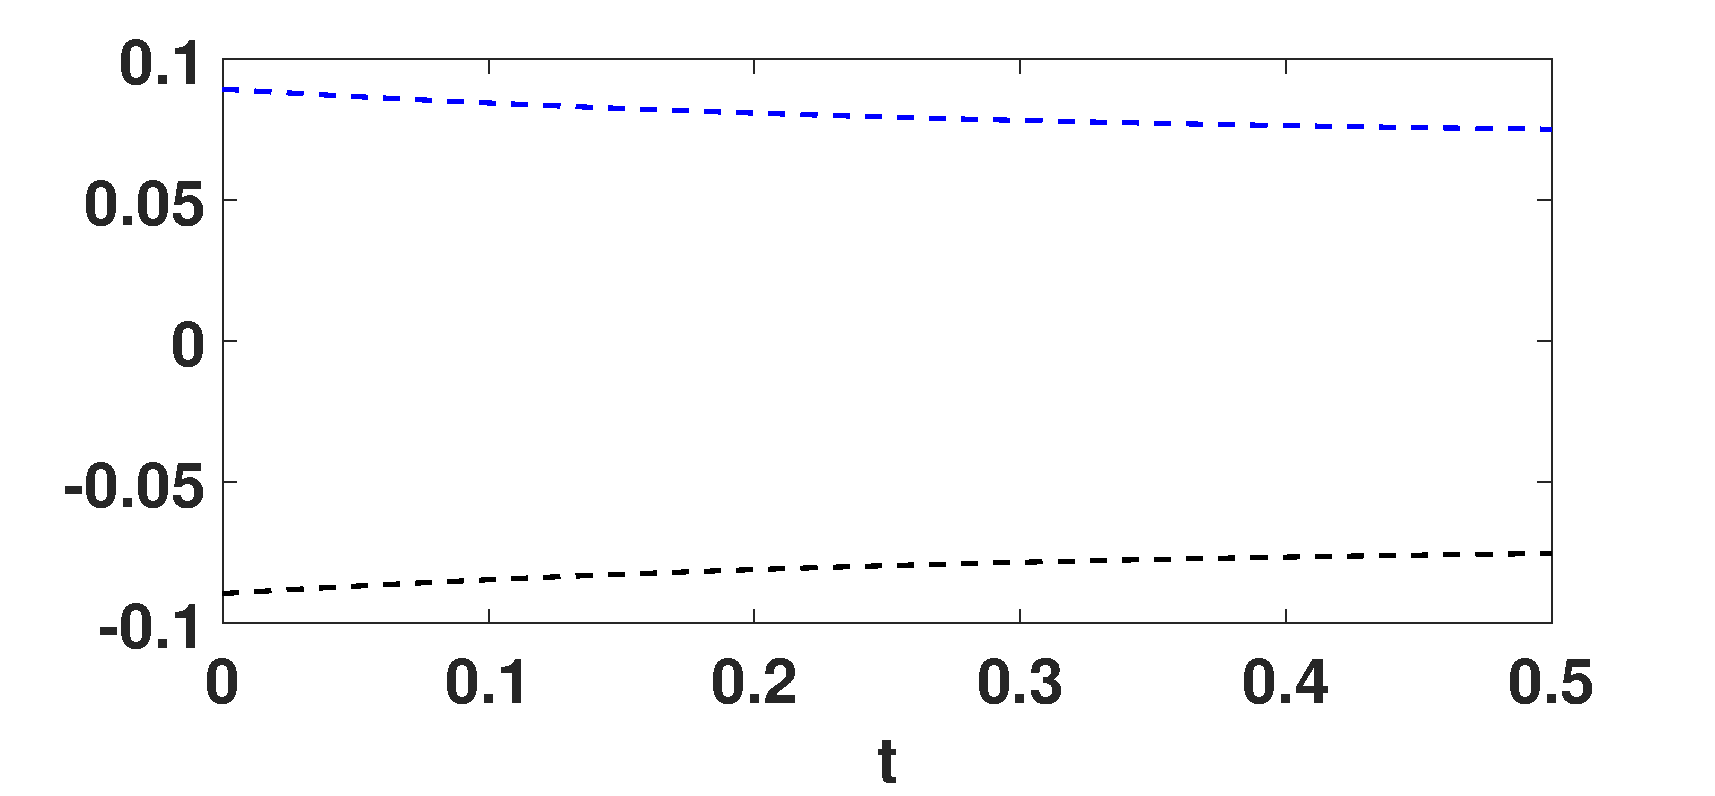
\includegraphics[width=.75\textwidth]{xtrack_mu_pt2_F_1_tf_pt5}
\caption{Horizontal positions of the two vortices for $0\leq t \leq .5$ for large Froude number $F=1$.}
\end{figure}
\begin{figure}[!h]
\centering
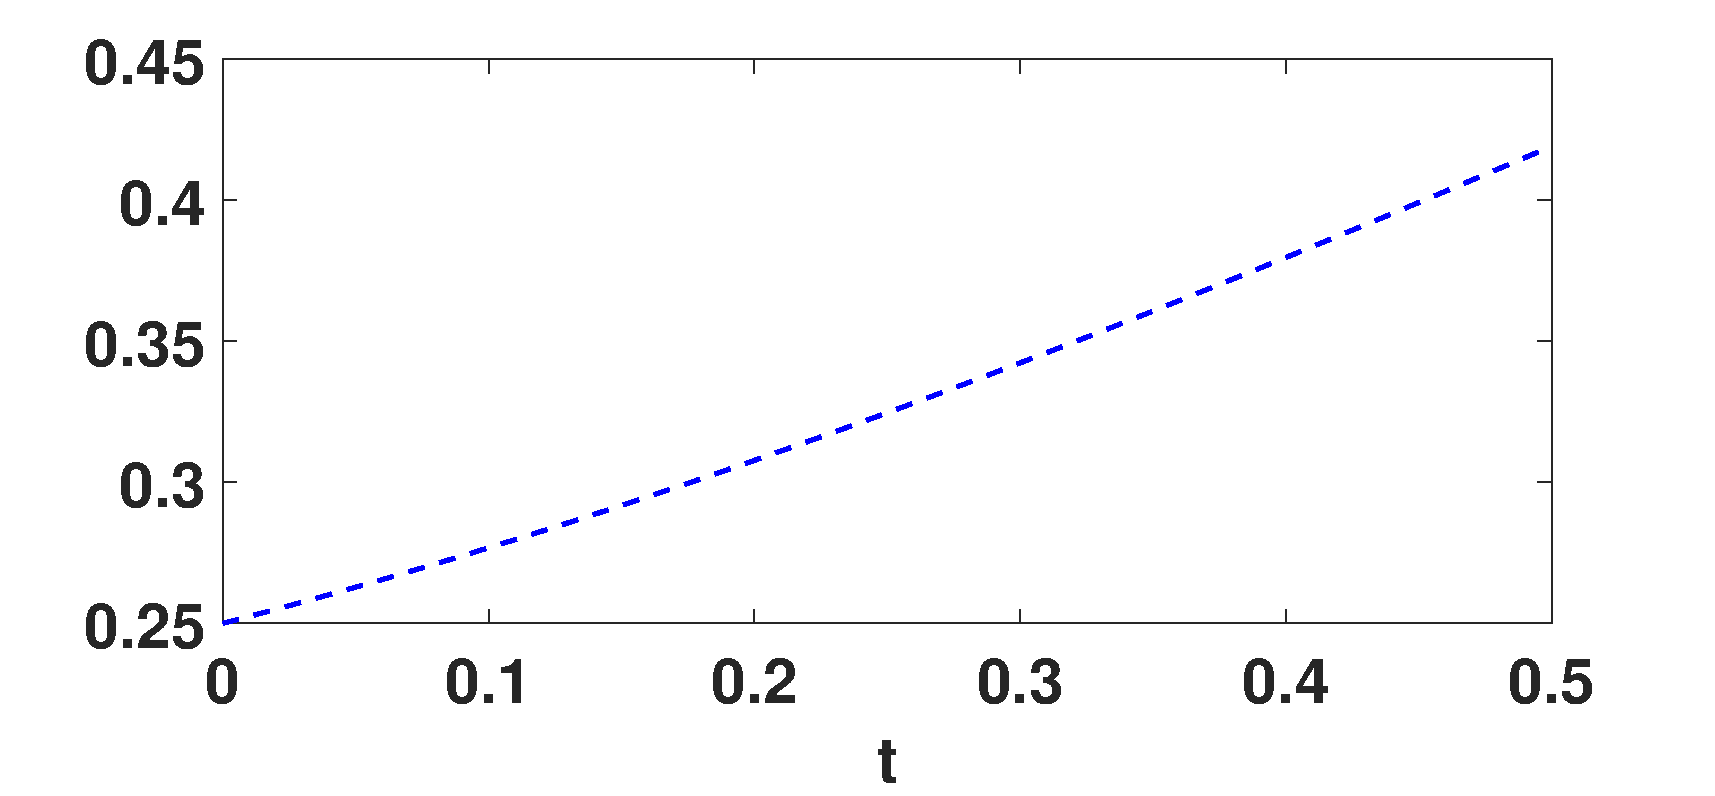
\includegraphics[width=.75\textwidth]{ztrack_mu_pt2_F_1_tf_pt5}
\caption{Vertical position of the two vortices for $0\leq t \leq .5$ for large Froude number $F=1$.}
\end{figure}

%%%%%%%%%%%%%%%%%%%%%%%%%%%%%%%%%%%%%%%%
\subsection*{Four Propagating Vortices: Plus/Plus,Minus/Minus}
Using the same numerical scheme and parameters as from above, we now look at the case of four vortices, chosen with vortex strengths
\[
\Gamma_{1}=\Gamma_{2}=1, ~ \Gamma_{3}=\Gamma_{4}=-1.
\]
We refer to this choice of vortex strengths as the `Plus/Plus,Minus/Minus' case.  The Froude number is set to $F=.2$.  In this case, the simulation can only be run to $t_{f}=.8$, after which vertical gradients appear in the surface profile signaling the possible onset of wave-breaking.  This is seen in Figure \ref{fig:surfrepppmm}, where one also sees high frequency oscillations indicative of unresolvable singularities in the profile.  This breakdown corresponds with what appears to be the first revolution of the vortices about one another as seen in Figure \ref{fig:xtrackppmm}.  This would seem to imply that while we described the case of $F=.2$ as weak above, the increased dynamics of the vortices appears to effectively increase their relative strength thereby inducing strongly nonlinear surface responses.   

\begin{figure}[!h]
\centering
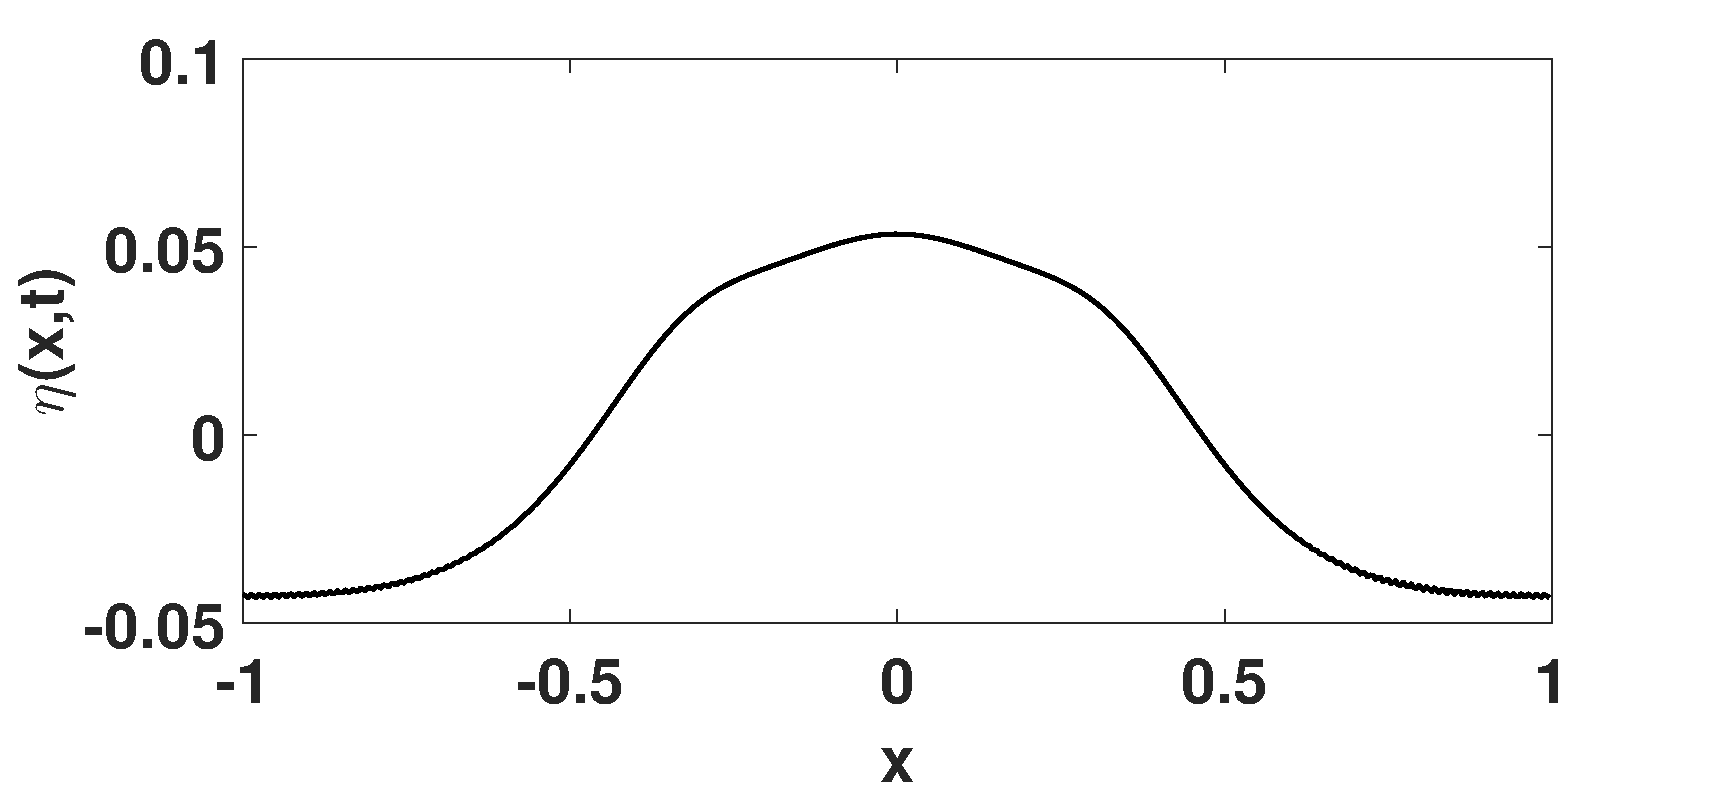
\includegraphics[width=.75\textwidth]{surf_resp_mu_pt2_F_pt2_tf_pt8_ppmm}
\caption{Surface response $\eta(x,.8)$ over four vortices in the Plus/Plus,Minus/Minus configuration.}
\label{fig:surfrepppmm}
\end{figure}
\begin{figure}[!h]
\centering
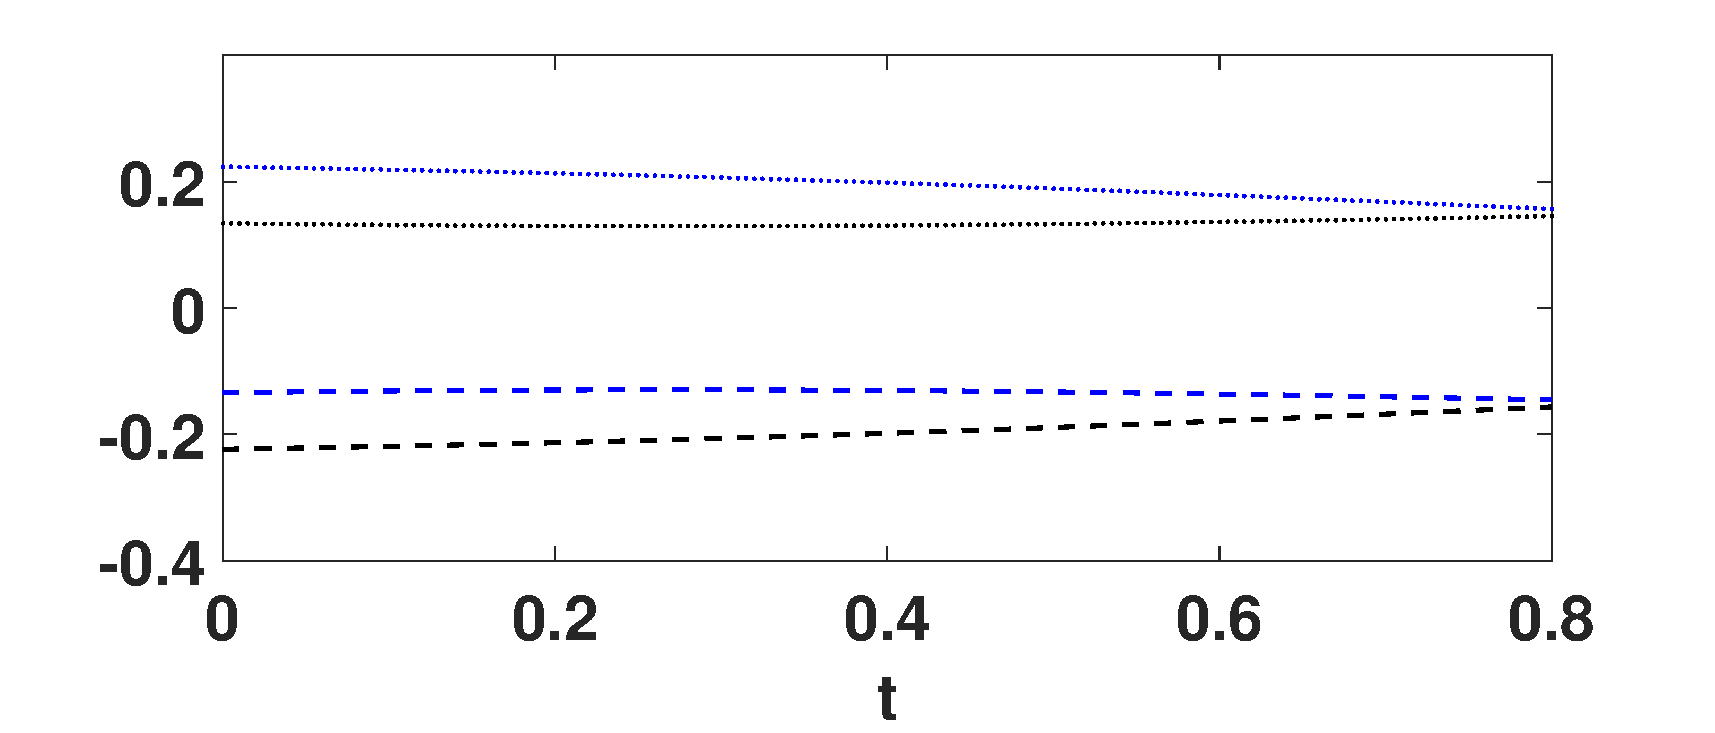
\includegraphics[width=.75\textwidth]{xtrack_mu_pt2_F_pt2_tf_pt8_ppmm}
\caption{Horizontal positions of four vortices in the Plus/Plus,Minus/Minus configuration for $0\leq t \leq .8$.}
\label{fig:xtrackppmm}
\end{figure}
\begin{figure}[!h]
\centering
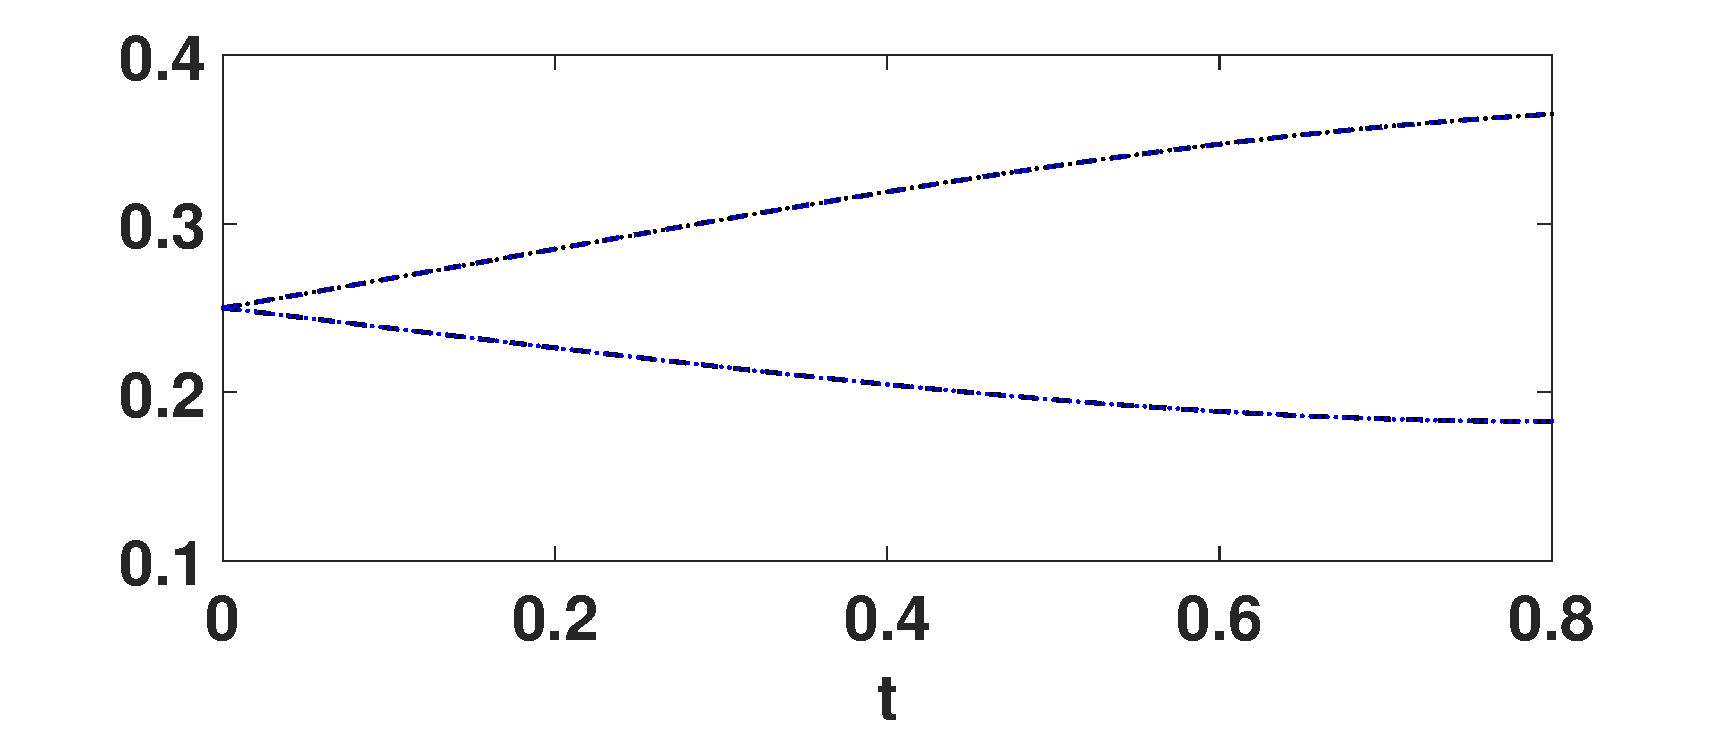
\includegraphics[width=.75\textwidth]{ztrack_mu_pt2_F_pt2_tf_pt8_ppmm}
\caption{Vertical position of four vortices in the Plus/Plus,Minus/Minus configuration for $0\leq t \leq .8$.}
\end{figure}
%%%%%%%%%%%%%%%%%%%%%%%%%%%%%%%%%%%%%%%%
\subsection*{Four Propagating Vortices: Plus/Minus,Minus/Plus}
We now examine the case of four vortices with vortex strengths chosen such that
\[
\Gamma_{1}=1, ~ \Gamma_{2}=-1, ~ \Gamma_{3}=-1,~\Gamma_{4}=1,
\]
which is why we refer to this case as `Plus/Minus,Minus/Plus'.  We choose $F=.2$, which, as pointed out in the previous section can be thought of as relatively strong when four vortices are present.  The simulation can be run to $t_{f}=3.5$ before high frequency phenomena causes the numerical method to break down, which we take the be a rough measure of the onset of wave breaking at the surface.  This can be clearly seen in Figure \ref{fig:surfreppmmp}, where jagged high frequency features can be seen in the asymmetric scars.  The presence of this asymmetry clearly corresponds to the markedly different paths of the vortices as seen in Figures \ref{fig:xtrackpmmp} and \ref{fig:ztrackpmmp}.
\begin{figure}[!h]
\centering
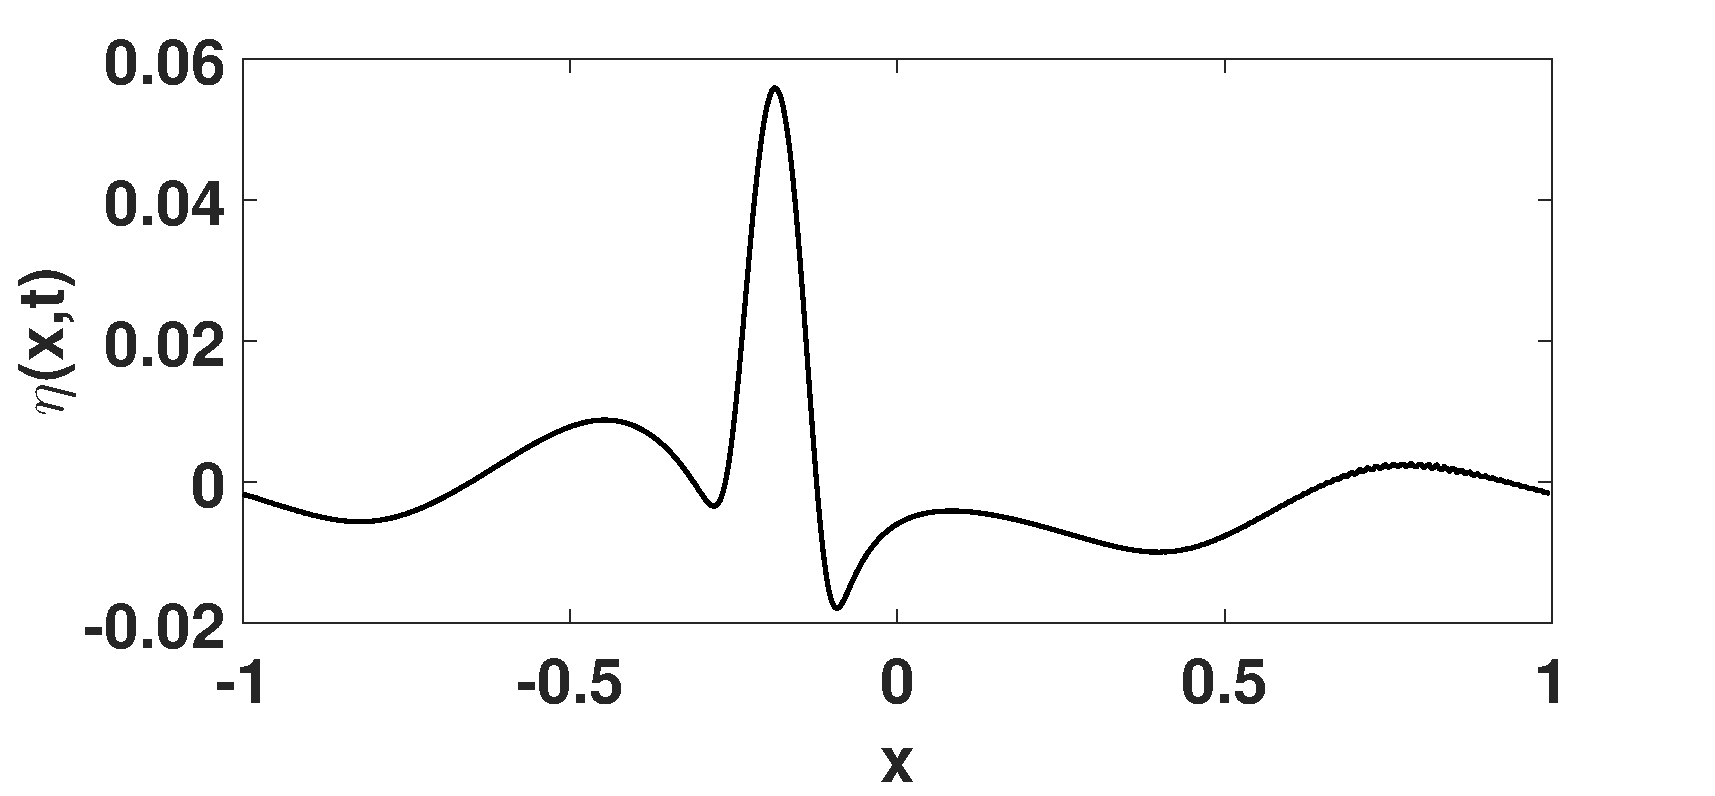
\includegraphics[width=.75\textwidth]{surf_resp_mu_pt2_F_pt2_tf_3pt5_pmmp}
\caption{Surface response $\eta(x,3.5)$ over four vortices in the Plus/Minus,Minus/Plus configuration.}
\label{fig:surfreppmmp}
\end{figure}
\begin{figure}[!h]
\centering
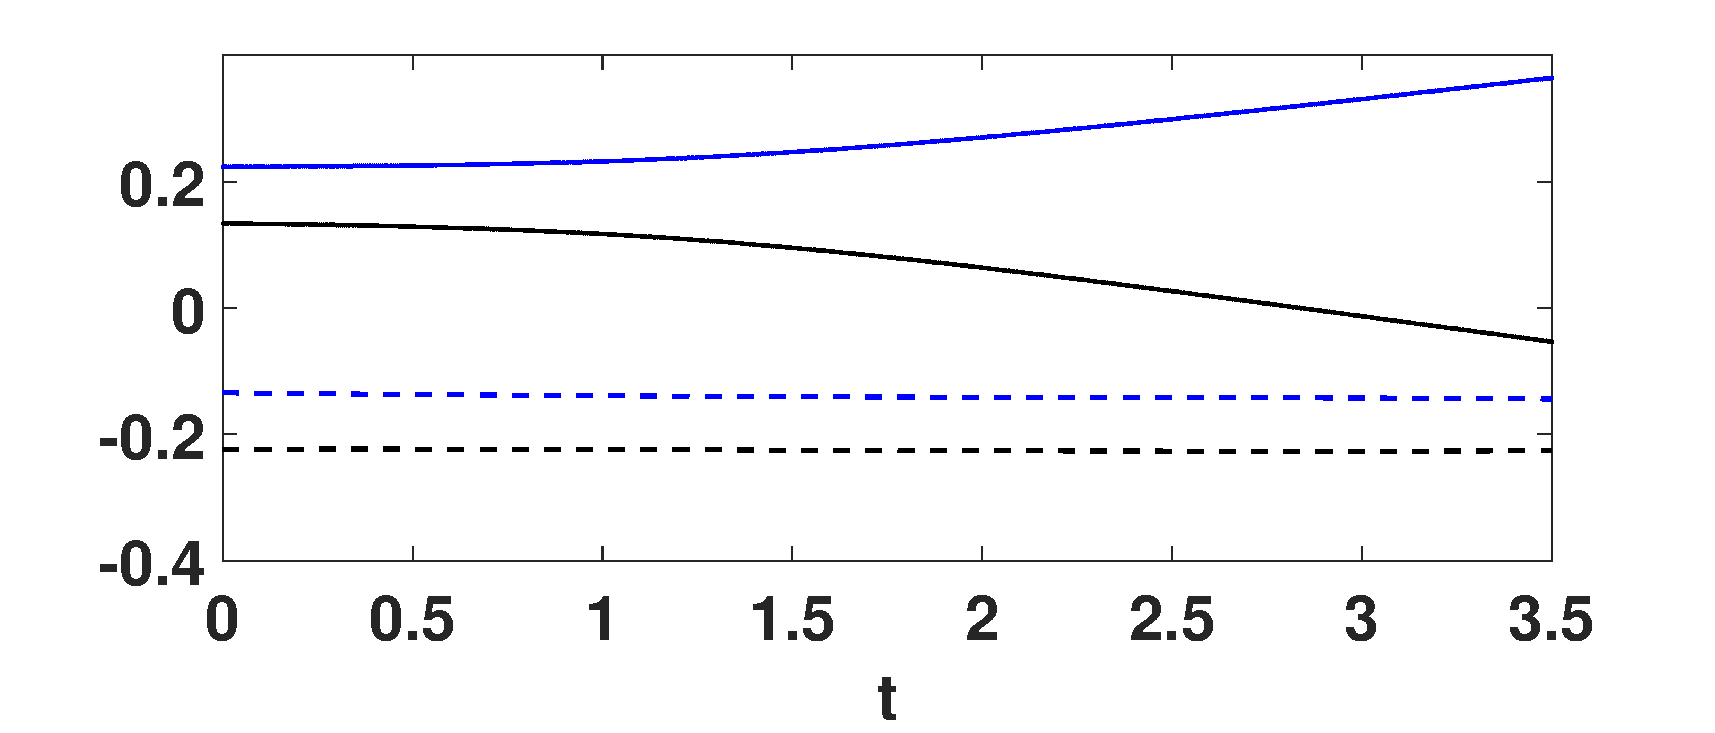
\includegraphics[width=.75\textwidth]{xtrack_mu_pt2_F_pt2_tf_3pt5_pmmp}
\caption{Horizontal positions of four vortices in the Plus/Minus,Minus/Plus configuration for $0\leq t \leq 3.5$.}
\label{fig:xtrackpmmp}
\end{figure}
\begin{figure}[!h]
\centering
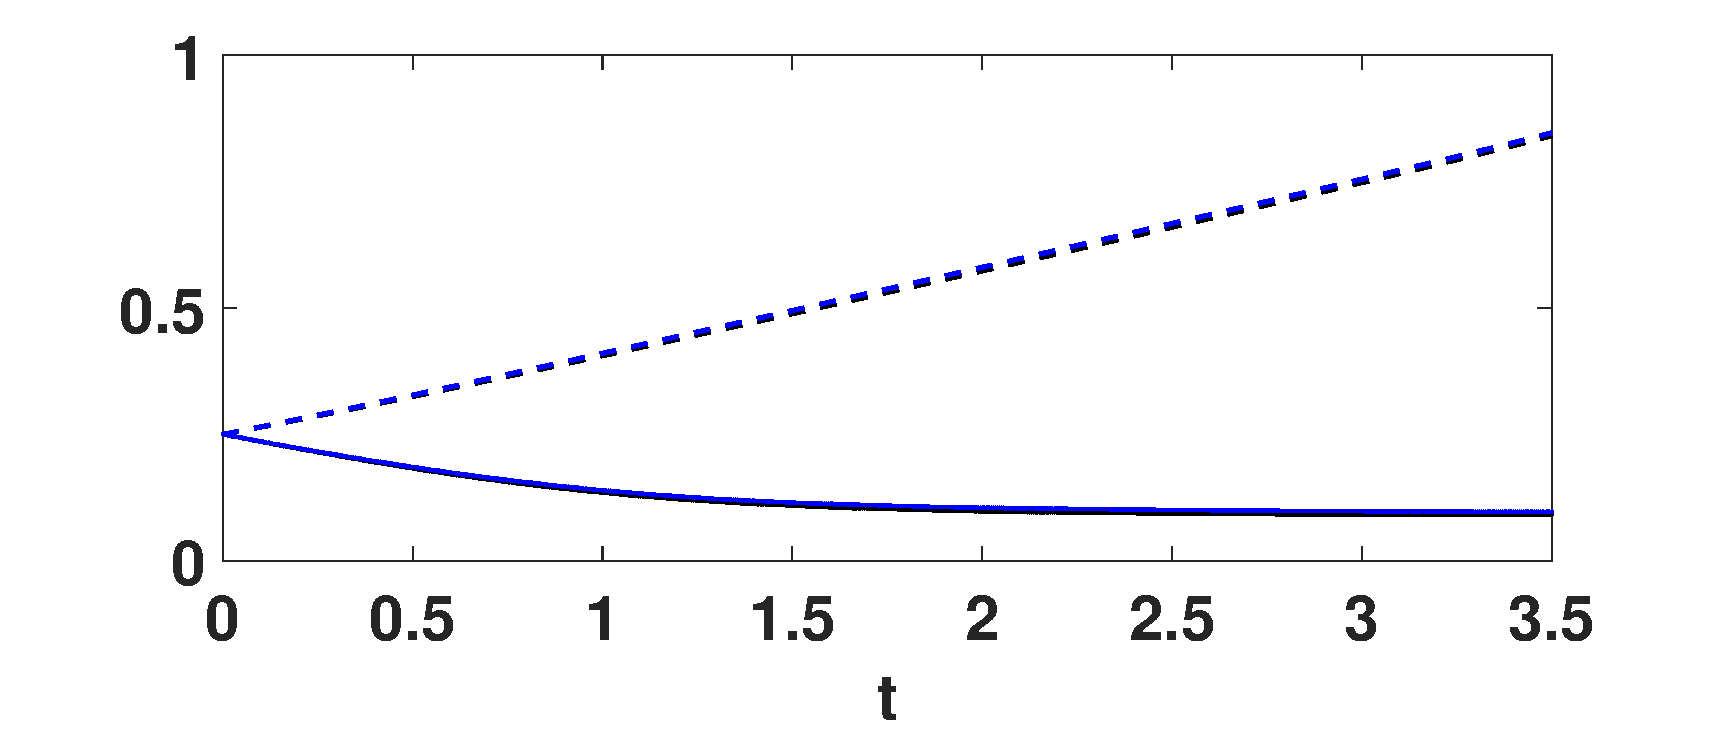
\includegraphics[width=.75\textwidth]{ztrack_mu_pt2_F_pt2_tf_3pt5_pmmp}
\caption{Vertical position of four vortices in the Plus/Minus,Minus/Plus configuration for $0\leq t \leq 3.5$.}
\label{fig:ztrackpmmp}
\end{figure}

%%%%%%%%%%%%%%%%%%%%%%%%%%%%%%%%%%%%%%%%
\subsection*{Four Propagating Vortices: Plus/Minus,Plus/Minus}
Finally, we now look at the case of four vortices, chosen so that
\[
\Gamma_{1}=1,~\Gamma_{2}=-1, ~ \Gamma_{3}=1,~\Gamma_{4}=-1.
\]
The Froude number is again set at $F=.2$.  In keeping with our convention, this is called the `Plus/Minus,Plus/Minus' case.  The simulation can be run to $t_{f}=4$ before high frequency phenomena causes the numerical method to break down, which we take the be a rough measure of the onset of wave breaking at the surface.  
\begin{figure}[!h]
\centering
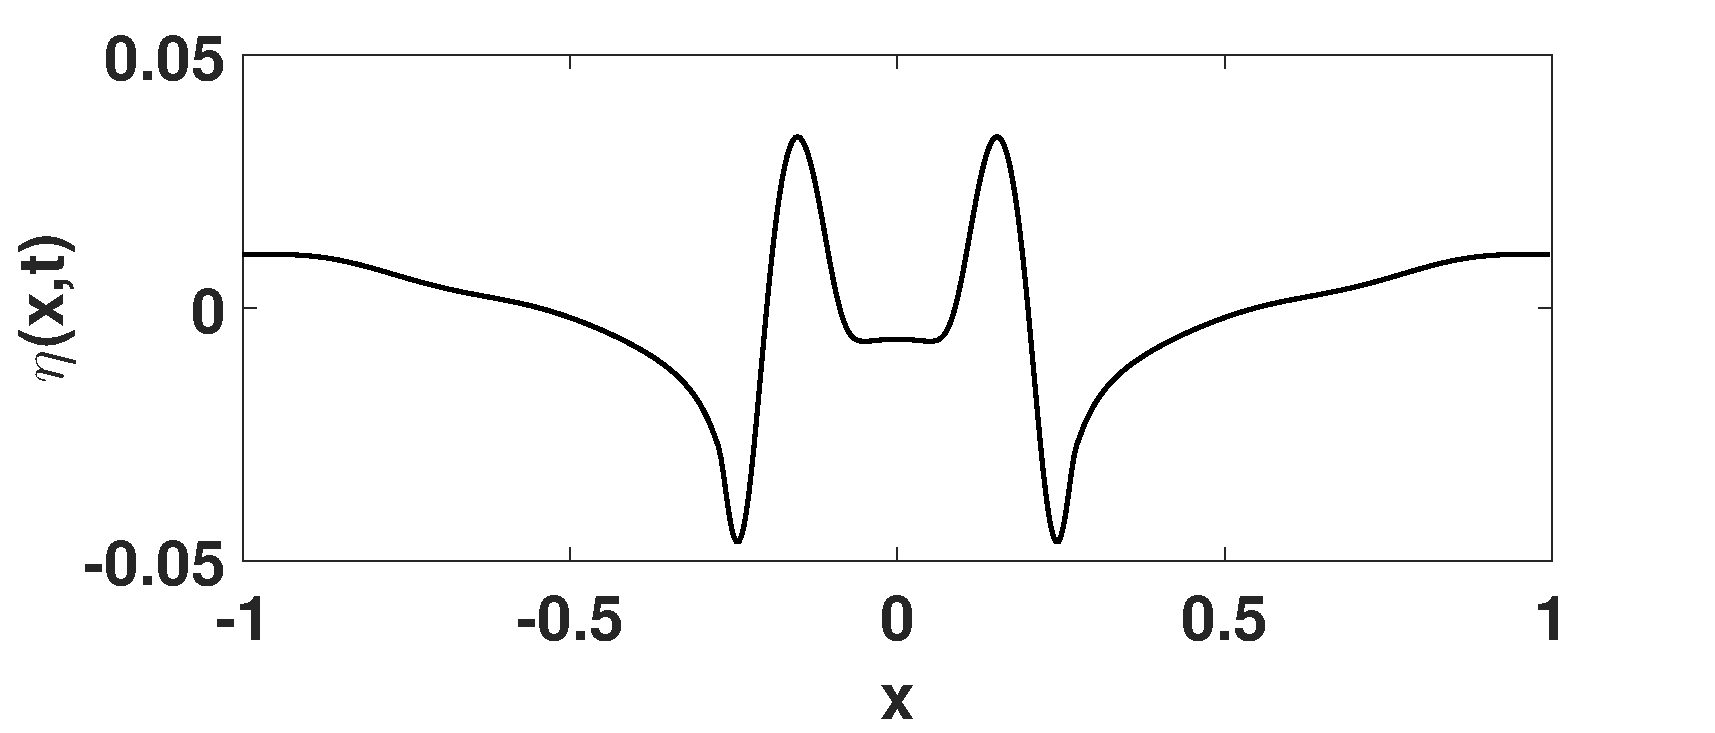
\includegraphics[width=.75\textwidth]{surf_resp_mu_pt2_F_pt2_tf_4pt2_pmpm}
\caption{Surface response $\eta(x,4)$ to four vortices in the Plus/Minus,Plus/Minus configuration.}
\label{fig:surfreppmpm}
\end{figure}
\begin{figure}[!h]
\centering
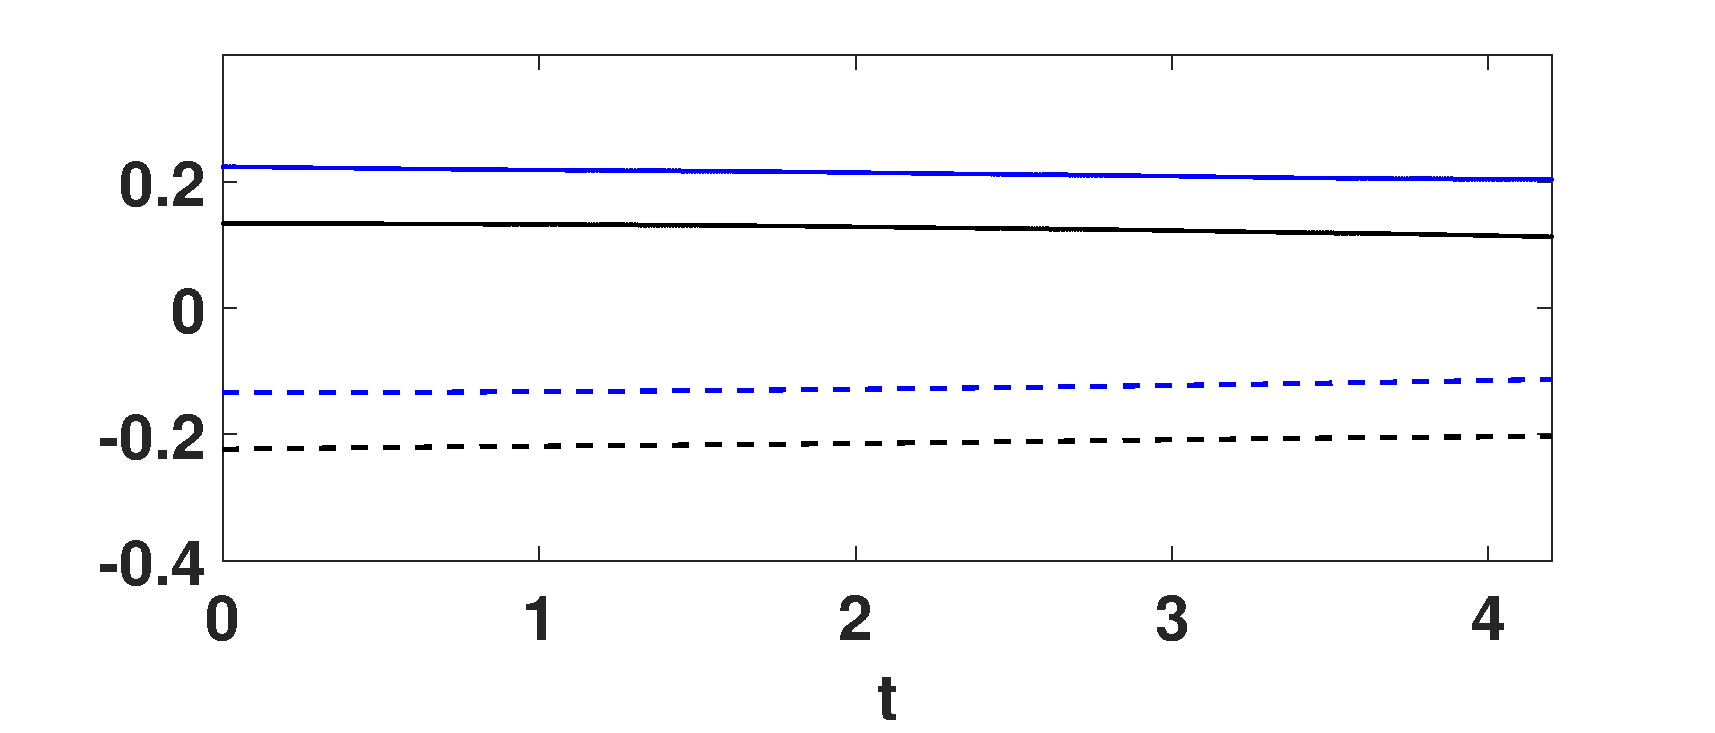
\includegraphics[width=.75\textwidth]{xtrack_mu_pt2_F_pt2_tf_4pt2_pmpm}
\caption{Horizontal positions of four vortices in the Plus/Minus,Plus/Minus configuration for $0\leq t \leq 4$.}
\end{figure}
\begin{figure}[!h]
\centering
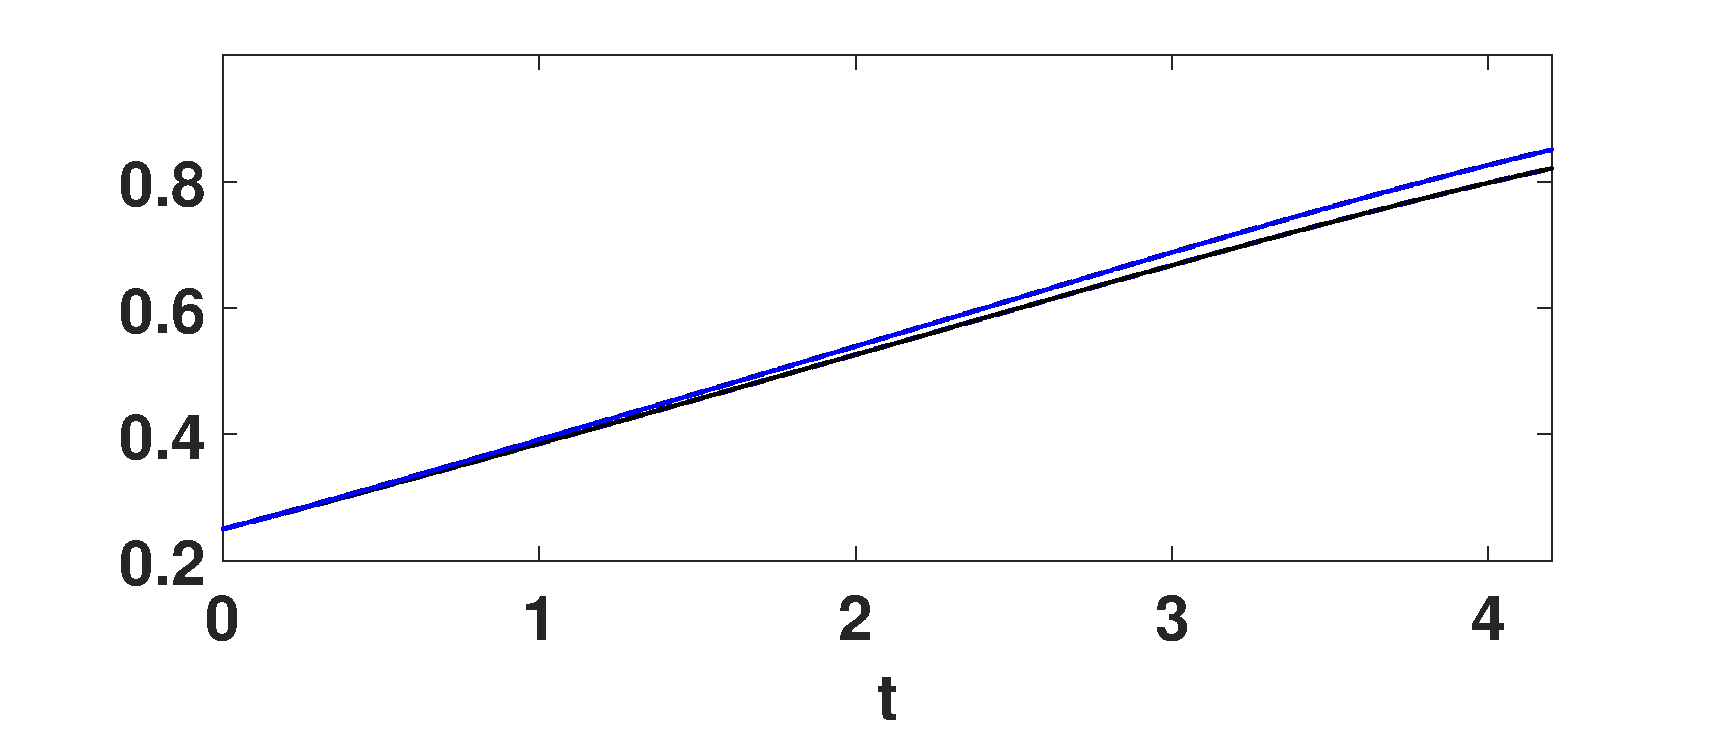
\includegraphics[width=.75\textwidth]{ztrack_mu_pt2_F_pt2_tf_4pt2_pmpm}
\caption{Vertical position of four vortices in the Plus/Minus,Plus/Minus configuration for $0\leq t \leq 4$.}
\end{figure}

%%%%%%%%%%%%%%%%%%%%%%%%%%%%%%%%%%%%%%%%%%%%%%%%%%%%%%%%%%%%%%%%%%%%%%%%%%%%%%%%
\section{Conclusion}

%%%%%%%%%%%%%%%%%%%%%%%%%%%%%%%%%%%%%%%%%%%%%%%%%%%%%%%%%%%%%%%%%%%%%%%%%%%%%%%%%%
\bibliography{waves_over_vortices}
\bibliographystyle{unsrt}
\end{document}